\documentclass[12pt,a4paper,2sides]{report}


\usepackage{lib/lib} %import libary from lib.sty %

%Thêm thư viện ở dưới dòng này.
\usepackage{mathptmx}
\onehalfspacing %Giãn dòng phân nửa.
%===============================
%Thêm dữ liệu vào intro.tex qua dòng lệnh.
%Addition into data at intro.tex file via command.
\newcommand{\khoa}{CÔNG NGHỆ THÔNG TIN} %TÊN NGÀNH, KHOA.
\newcommand{\bai}{BÁO CÁO CUỐI KỲ}
\newcommand{\de}{XÂY DỰNG VÀ PHÁT TRIỂN HỆ THỐNG MUA SẮM THỜI TRANG TRỰC TUYẾN}
\newcommand{\monhoc}{PHÁT TRIỂN HỆ THỐNG THÔNG TIN DOANH NGHIỆP} %TÊN MÔN HỌC 
\newcommand{\gvhd}{Ths.Dương Hữu Phúc} %TÊN CỦA GIẢNG VIÊN HƯỚNG DẪN
\newcommand{\tacgia}{Nguyễn Thị Thảo Như} %TÊN CỦA NGƯỜI VIẾT
\newcommand{\mstacgia}{51900162} %MÃ SỐ SINH VIÊN
\newcommand{\svhai}{Lê Trí Đức}
\newcommand{\msvhai}{51900040}
\newcommand{\svba}{Nguyễn Quốc Hợp}
\newcommand{\msvba}{51900745}
\newcommand{\svtu}{}
\newcommand{\msvtu}{}
\newcommand{\nam}{2022}
%Acknowledge page (the second page in docs)
\newcommand{\loicamon}{
		Với những kiến thức em tích lũy được qua những ngày học tập, đây là kết quả của quá trình học tập của em và nhóm cùng đưa ra ý kiến và thảo luận, tổng hợp kiến thức lại với nhau.\\
}
%tabl
\begin{document}	
\pagenumbering{roman}
% \begin{center}
	\large{\textbf{TỔNG LIÊN ĐOÀN LAO ĐỘNG VIỆT NAM}} \\
	\large{\textbf{TRƯỜNG ĐẠI HỌC TÔN ĐỨC THẮNG}} \\
	\large{\textbf{\MakeUppercase{KHOA \khoa}}} \\\vspace*{1cm}	
	
\includegraphics[width=0.5\linewidth]{lib/TDTlogo.jpg}\\\vspace*{1cm}	
	\Large{\textbf{\MakeUppercase{\bai}}}\\		
	\LARGE{\textbf{\MakeUppercase{\de}}}\\
	\Large{\textbf{\MakeUppercase{\monhoc}}}\vspace*{1.5cm}
\begin{flushright}			

	\large{\textit{Người thực hiện:}} \\
	\large{\textbf{\tacgia}}\\
	\large{\textbf{\mstacgia}}\\
	\large{\textbf{\svhai}}\\
	\large{\textbf{\msvhai}}\\
	\large{\textbf{\svba}}\\
	\large{\textbf{\msvba}}\\
	\large{\textit{Giảng viên hướng dẫn:}} \\
	\large{\textbf{\gvhd}} 
	\vspace*{1.5cm}
\end{flushright}
	\large{\textbf{Thành phố Hồ Chí Minh, \nam.}}
\end{center}	
	\newpage
\begin{center}
	\Large{\textbf{LỜI CẢM ƠN}}
\end{center}

	Em xin được gửi lời cảm ơn đến giảng viên \gvhd \mbox{} đã tận tình giảng dạy và giúp đỡ em trong việc hoàn thành bài tập, cũng như hiểu vấn đề của môn học đề ra.\\
	
	Với những kiến thức em tích lũy được qua những ngày học tập, đây là kết quả của quá trình học tập của em. Tuy vẫn còn nhiều mặt còn hạn chế, nhưng em sẽ cố gắng để đạt được kết quả tốt nhất có thể.\\
	\newpage
\begin{center}
	\Large{\textbf{BÀI TIỂU LUẬN ĐƯỢC HOÀN THÀNH}} \\
	\Large{\textbf{TẠI TRƯỜNG ĐẠI HỌC TÔN ĐỨC THẮNG}} \\
\end{center}	
Em xin cam đoan đây là bài báo cáo sản phẩm \bai \mbox{} của chỉ riêng em. Các nội dung nghiên cứu, kết quả trong đề tài này là trung thực và chưa được công bố dưới bất kỳ hình thức nào. Những số liệu trong các bảng biểu phục vụ cho việc phân tích, nhận xét, đánh giá được chính tác giả thu thập từ các nguồn khác nhau có ghi rõ trong phần tài liệu tham khảo.\\

Ngoài ra, trong đề tài còn sử dụng một số nhận xét, đánh giá cũng như số liệu của các tác giả khác, cơ quan tổ chức khác đều có trích dẫn và chú thích nguồn gốc rõ ràng và cụ thể.\\

Nếu phát hiện có bất kỳ sự gian lận nào em xin hoàn toàn chịu trách nhiệm về nội dung của bài \bai. Trường đại học Tôn Đức Thắng không liên quan đến những vi phạm tác quyền trong quá trình thực hiện của em.\\

\begin{center}
	\hspace*{7cm}Trường ĐH Tôn Đức Thắng,\\
	\hspace*{7cm}Ngày ........ tháng ........ năm \nam.\\
	\hspace*{7cm}Sinh viên thực hiện,\\
	\hspace*{7cm}(Ký và ghi rõ họ tên)\\
	\vspace*{0.2cm}
	\vspace*{2cm}
	 %
\includegraphics[width=0.7\linewidth]{lib/signate.png}\\
	\hspace*{7cm}\tacgia.
\end{center}		
	\newpage
\begin{center}
	\Large{\textbf{PHẦN XÁC NHẬN VÀ ĐÁNH GIÁ}}
\end{center}
	\textbf{Phần đánh giá của giảng viên chấm bài:}\\
	...............................................................................................................................................\\
	...............................................................................................................................................\\
	...............................................................................................................................................\\
	...............................................................................................................................................\\
	...............................................................................................................................................\\
	...............................................................................................................................................\\
	...............................................................................................................................................\\
	...............................................................................................................................................\\
	...............................................................................................................................................
\begin{center}
	\hspace*{5cm} TP. Hồ Chí Minh, ngày..... tháng..... năm \nam.\\
	\hspace*{5cm} Giảng viên chấm bài,\\
	\vspace*{1.2cm}
	\hspace*{5cm} .......................................
\end{center}
	\vspace*{0.5cm}
	\textbf{Phần đánh giá của giảng viên hướng dẫn:}\\
	...............................................................................................................................................\\
	...............................................................................................................................................\\
	...............................................................................................................................................\\
	...............................................................................................................................................\\
	...............................................................................................................................................\\
	...............................................................................................................................................\\
	...............................................................................................................................................\\
	...............................................................................................................................................\\
	...............................................................................................................................................
\begin{center}
	\hspace*{5cm} TP. Hồ Chí Minh, ngày..... tháng..... năm \nam.\\
	\hspace*{5cm} Giảng viên hướng dẫn,\\
	\vspace*{2cm}
	\hspace*{5cm} \gvhd.
\newpage
\end{center}

\begin{center}
	\large{\textbf{TỔNG LIÊN ĐOÀN LAO ĐỘNG VIỆT NAM}} \\
	\large{\textbf{TRƯỜNG ĐẠI HỌC TÔN ĐỨC THẮNG}} \\
	\large{\textbf{\MakeUppercase{KHOA \khoa}}} \\\vspace*{1cm}	
	
\includegraphics[width=0.5\linewidth]{lib/TDTlogo.jpg}\\\vspace*{1cm}	
	\Large{\textbf{\MakeUppercase{\monhoc}}}\vspace*{0.5cm}\\
	\Large{\textbf{\MakeUppercase{\bai}}}\\		
	\LARGE{\textbf{\MakeUppercase{\de}}}\vspace*{2cm}\\

\begin{flushright}			
	\large{\textit{Giảng viên hướng dẫn:}}
	\large{\textbf{\gvhd}} \\
	\large{\textit{Người thực hiện:}} 
	\large{\textbf{\tacgia}}
	\large{\textbf{\mstacgia}}\\
	\large{\textbf{\svhai}}
	\large{\textbf{\msvhai}}\\
	\large{\textbf{\svba}}
	\large{\textbf{\msvba}}\\

	\vspace*{1.5cm}
\end{flushright}
	\large{\textbf{Thành phố Hồ Chí Minh, \nam.}}
\end{center}	
	\newpage
\begin{center}
	\Large{\textbf{LỜI CẢM ƠN}}
\end{center}

Trước tiên với tình cảm sâu sắc và chân thành nhất, cho phép chúng em được bày tỏ lòng biết ơn đến quý thầy/cô trường Đại học Tôn Đức Thắng đã cùng với tri thức và tâm huyết của mình để truyền đạt vốn kiến thức quý báu cho chúng em trong suốt học kỳ vừa rồi.

Chúng em xin tỏ lòng biết ơn sâu sắc đến giảng viên \gvhd \mbox{} đã tận tâm hướng dẫn chúng em qua từng buổi học và cũng là người tận tình hướng dẫn, giúp đỡ trong suốt quá trình hoàn thành bài báo cáo này.

Với điều kiện thời gian cũng như kinh nghiệm còn hạn chế của sinh viên, bài báo cáo này không thể tránh được những thiếu sót. Nhóm chúng em rất mong nhận được sự chỉ bảo, đóng góp ý kiến của các quý thầy/cô để em có điều kiện bổ sung, nâng cao kiến thức, kinh nghiệm của mình.

\hspace{8cm}Tập thể nhóm xin chân thành cảm ơn!

	\newpage
\begin{center}
	\Large{\textbf{BÀI TIỂU LUẬN ĐƯỢC HOÀN THÀNH}} \\
	\Large{\textbf{TẠI TRƯỜNG ĐẠI HỌC TÔN ĐỨC THẮNG}} \\
\end{center}	

Em xin cam đoan đây là bài báo cáo sản phẩm \bai \mbox{} của chỉ riêng em. Các nội dung nghiên cứu, kết quả trong đề tài này là trung thực và chưa được công bố dưới bất kỳ hình thức nào. Những số liệu trong các bảng biểu phục vụ cho việc phân tích, nhận xét, đánh giá được chính tác giả thu thập từ các nguồn khác nhau có ghi rõ trong phần tài liệu tham khảo.\\

Ngoài ra, trong đề tài còn sử dụng một số nhận xét, đánh giá cũng như số liệu của các tác giả khác, cơ quan tổ chức khác đều có trích dẫn và chú thích nguồn gốc rõ ràng và cụ thể.\\

Nếu phát hiện có bất kỳ sự gian lận nào em xin hoàn toàn chịu trách nhiệm về nội dung của bài \bai. Trường đại học Tôn Đức Thắng không liên quan đến những vi phạm tác quyền trong quá trình thực hiện của em.\\

\begin{center}
	\hspace*{7cm}Trường ĐH Tôn Đức Thắng,\\
	\hspace*{7cm}Ngày ...30... tháng ...11... năm \nam.\\
	\hspace*{7cm}Sinh viên thực hiện,\\
	\hspace*{7cm}(Ký và ghi rõ họ tên)\\
	\vspace*{0.2cm}
	\vspace*{2cm}
	 %
\includegraphics[width=0.7\linewidth]{lib/signate.png}\\
	\hspace*{7cm}\tacgia.
\end{center}		
	\newpage
\begin{center}
	\Large{\textbf{PHẦN XÁC NHẬN VÀ ĐÁNH GIÁ}}
\end{center}
	\textbf{Phần đánh giá của giảng viên chấm bài:}\\
	...............................................................................................................................................\\
	...............................................................................................................................................\\
	...............................................................................................................................................\\
	...............................................................................................................................................\\
	...............................................................................................................................................\\
	...............................................................................................................................................\\
	...............................................................................................................................................\\
	...............................................................................................................................................\\
	...............................................................................................................................................
\begin{center}
	\hspace*{5cm} TP. Hồ Chí Minh, ngày..30.. tháng..11... năm \nam.\\
	\hspace*{5cm} Giảng viên chấm bài,\\
	\vspace*{1.2cm}
	\hspace*{5cm} .......................................
\end{center}
	\vspace*{0.5cm}
	\textbf{Phần đánh giá của giảng viên hướng dẫn:}\\
	...............................................................................................................................................\\
	...............................................................................................................................................\\
	...............................................................................................................................................\\
	...............................................................................................................................................\\
	...............................................................................................................................................\\
	...............................................................................................................................................\\
	...............................................................................................................................................\\
	...............................................................................................................................................\\
	...............................................................................................................................................
\begin{center}
	\hspace*{5cm} TP. Hồ Chí Minh, ngày ..30.. tháng..11.. năm \nam.\\
	\hspace*{5cm} Giảng viên hướng dẫn,\\
	\vspace*{2cm}
	\hspace*{5cm} \gvhd.
\newpage
\end{center}

\newpage
\clearpage
%--------------Mục lục
\dominitoc
\tableofcontents %pages
%if you want to show table of contents of chapter, set \dominitoc under line \chapter{name}
%\listoffigures %pictures
\newpage
\clearpage
%\setcounter{page}{-1}
%\listoftables
%\begin{figure/tables}
%\centering
%Sourcode/Import
%\caption
%\end{fugure/tables}
\clearpage
\pagenumbering{arabic}
\setcounter{page}{1}
\clearpage
%\Control to file to create subfile.\\
%\chapter{Tóm tắt \& giới thiệu}
\minitoc
\newpage
\section{Giới thiệu đề tài}
\subsection{Mô tả đề tài}
\lipsum[1-4] %Thử với đoạn text này chơi.\textsl{}




% \minitoc
\newpage
\chapter{Tổng quan đề tài}
\section{Lý do chọn đề tài} 
Hòa vào nhịp điệu phát triển của thế giới, ngành thời trang của Việt Nam ta đang trên đà lớn mạnh. Làm đẹp đang dần trở thành nhu cầu thiết yếu trong đời sống của mọi người. Khi mức sống của người dân ngày càng được nâng cao thì nhu cầu về mua sắm và làm đẹp của họ cũng tăng. Quần áo đang ngày càng được quan tâm và việc mua sắm quần áo đã dần gắn liền với hoạt động của mỗi người, đôi lúc nó là một hoạt động thư giãn sau những khoảng thời gian mệt mỏi, sau những buổi đi làm, đi học. Do đó, thời trang luôn là một trong những ngành hàng kinh doanh mang lại doanh thu nhiều nhất.

Đối với lĩnh vực kinh doanh thời trang truyền thống, chủ cửa hàng có thể sử dụng một văn phòng chứa đầy những sổ sách lưu trữ dữ liệu cũng như giám sát tất cả các hoạt động kinh doanh và phân phối sản phẩm hằng ngày của cửa hàng. Tuy nhiên nếu họ muốn tìm một cách thức kinh doanh có thể làm tăng số lượng người mua, sản phẩm dễ dàng thu hút nhiều người dùng hơn cũng như giảm đi nhiều những chi phí tổ chức kinh doanh và làm tăng lợi nhuận cho cửa hàng thì ecommerce website chính là lựa chọn tốt nhất dành cho họ.

Internet chính là một nền tảng mạnh mẽ khiến cho lĩnh vực kinh doanh ngày càng được mở rộng. Có hàng triệu người dùng tìm kiếm sản phẩm và dịch vụ mà họ cần. Mua sắm trực tuyến đang tăng lên hàng nằm và đây được coi là một phương pháp thuận tiện để mua sản phẩm, nơi ai cũng có thể mua bất cử lúc nào, bất cứ nơi đâu.

Hình thức bán hàng trực tuyến cho phép người mua và người bán tiếp xúc với nhau một cách dễ dàng, kết nối không giới hạn. Hơn nữa, e-commerce cho phép tiết kiệm được các khoản chi phí trong bán hàng, giúp cắt giảm các khâu bán hàng không cần thiết, nhờ đó mang đến một mức giá tốt hơn cho người mua. Điều quan trọng hơn, ecommerce website còn cho phép chủ cửa hàng sử dụng một loạt các kỹ thuật tiếp thị và bán hàng để cung cấp cho mọi người thêm lý do để ở lại trên trang web và khiến họ mua sản phẩm của cửa hàng nhiều hơn.

Việc tích hợp lĩnh vực kinh doanh thời trang vào Ecommerce website là một điều không hề đơn giản. Những nhà phát triển hệ thống luôn phải tìm hiểu, phân tích để có thể chuyển mô hình kinh doanh truyền thống thành một mô hình kinh doanh tự động và chuyển chúng sang một hệ thống thông tin chính xác và đầy đủ nhất.

Chính vì thế, thực hiện đề tài “Xây dựng và phát triển hệ thống quản lý quy trình mua sắm thời trang trực tuyến” sẽ tạo nên một nền tảng để nhóm có thể học tập và rèn luyện để có cái nhìn tổng quan đối với những vấn đề đang xảy ra ở thực tế.
\section{Mục tiêu chọn đề tài} 
Mục tiêu chung của việc thực hiện đồ án này nhằm tìm hiểu về quy trình mua bán trong hệ thống thông tin quản lý mua sắm thời trang trực tuyến B2C bằng việc vận dụng các kiến thức đã học từ bộ môn Phát Triển Hệ Thống Thông Tin Doanh Nghiệp và tự tìm hiểu về ngành thương mại điện tử nói chung cũng như là quy trình đặt hàng và xử lý đơn hàng của hệ thống nói riêng.
\section{Phạm vi đề tài} 
Đề tài: "Xây dựng và phát triển quy trình mua sắm thời trang trực tuyến"
Phạm vi các sản phẩm phần mềm đề xuất sẽ đáp ứng trong đề tài bao gồm các quy trình sau:
\begin{itemize}
    \item Mua hàng
    \item Xử lý đơn hàng
    \item Xử lý sau bán hàng
\end{itemize}
Phần mềm đáp ứng đầy đủ nhu cầu mua sắm của khách hàng cũng như giúp cho phía cửa hàng thời trang có thể dễ dàng quản lý sản phẩm, đơn hàng của họ. 
Trong quá trình thực hiện, nhóm ghi nhận được một số điều kiện nghiệm thu:
\begin{itemize}
    \item Cửa hàng mong muốn hệ thống có thể lưu trữ giá sản phẩm sau khi giảm giá trong hóa đơn của khách hàng tại thời điểm mua hàng
    \item Một số sản phẩm trong cửa hàng sẽ được định giá tùy theo màu sắc của nó, có một vài màu sắc giới hạn sẽ được kê giá cao hơn các màu sắc bình thường khác
    \item Cửa hàng mong muốn có thể quản lý được các trạng thái được cập nhật bởi nhân viên nào và tại thời điểm nào.
\end{itemize}
Phương án xử lý sau khi hệ thống trong quá trình nghiệm thu gặp phải những vấn đề trên:
\begin{itemize}
    \item Trong hóa đơn của khách hàng sẽ lưu trữ hai loại giá cả là giá mặc định và giá sau khi giảm 
    \item Mỗi màu sắc của sản phẩm trong hệ thống sẽ cho phép cửa hàng thêm một mức giá cố định, ví dụ: một sản phẩm sau khi đã tính toán hết các chi phí sẽ cho ra một giá bán là 500.000 VND, tuy nhiên màu trắng của sản phẩm đó có giá là 200.000 VND. Như vậy hệ thống sẽ tính ra giá bán cuối cùng cho sản phẩm có màu trắng là 700.000 VND
    \item Khi nhân viên cập nhật trạng thái, hệ thống sẽ lưu trữ lại thông tin đầy đủ về nhân viên, thời gian cập nhật
\end{itemize}
\section{Ý nghĩa đề tài}
Tùy theo cách nhìn nhận vấn đề quản lý quy trình bán hàng trực tuyến mà có những cách hiểu và cách giải quyết khác nhau. Do vậy, khi nghiên cứu sâu và xây dựng đề tài giúp chúng ta có thể nhìn nhận vấn đề từ nhiều góc độ khác nhau để biết được đâu là những hoạt động quan trọng trong quy trình cũng như có thể tối ưu hóa quy trình kinh doanh truyền thống sang một quy trình tự động tối ưu hơn, nhanh hơn, đạt nhiều lợi nhuận hơn.

Chuyển đổi mô hình kinh doanh sang một hệ thống thông tin tự động không chỉ giúp doanh nghiệp dễ dàng tiếp cận được nhiều khách hàng ở xa mà còn có thể giúp doanh nghiệp quản lý lượng dữ liệu được sinh ra mỗi ngày. Việc chuyển đổi này giúp doanh nghiệp đẩy nhanh được quá trình hội nhập kinh tế, từ đó mới phát huy hết khả năng của mình và hạn chế những bất hợp lý để đưa doanh nghiệp ngày càng phát triển.


\chapter{Phân tích và thiết kế hệ thống}
\section{Phân tích quy trình kinh doanh}
\subsection{Tìm hiểu quy trình thực tế:}
Các bước trong quy trình mua sắm của khách tại cửa hàng:
\begin{itemize}
    \item Khách hàng vào cửa hàng mua sắm
    \item Trợ lý bán hàng sẽ tư vấn vị trí của các mặt hàng mà khách hàng cần tìm
    \item Khách hàng đi lấy xe đẩy chứa hàng
    \item Khách hàng lựa chọn sản phẩm và cho vào xe đẩy
    \item Khách hàng đẩy giỏ hàng đến quầy thanh toán
    \item Khách hàng chờ đợi được thanh toán
    \item Khách hàng thực hiện thanh toán
\end{itemize}
\subsection{Quy trình nghiệp vụ trong hệ thống}
Từ quy trình mua sắm thực tế, ta tiến hành chuyển đổi sang các quy trình nghiệp vụ mà hệ thống sẽ hỗ trợ. 
\subsubsection{Mua hàng}
Bước 1: Tạo giỏ hàng 

Một khách hàng không cần phải đăng ký, đăng nhập trên trang web khi ghé thăm và xem các sản phẩm của cửa hàng. Quy trình đặt hàng chỉ thực sự bắt đầu ngay khi khách hàng chọn một sản phẩm và thêm nó vào giỏ hàng. Khách hàng bắt buộc phải đăng nhập tài khoản để có thể thực hiện quy trình đặt hàng.

Sản phẩm được chọn sẽ lưu vào trong giỏ hàng tương ứng với mỗi khách hàng và có thể được xem lại. Nếu khách hàng không hoàn thành thủ tục thanh toán thì các sản phẩm vẫn được lưu trữ trong giỏ hàng.

Trường hợp sản phẩm đã bán hết thì mặt hàng đó trong giỏ hàng của khách sẽ chuyển sang trạng thái hết hàng. Khi khách hàng trở lại trang web, giỏ hàng vẫn đảm bảo chứa các sản phẩm để khách hàng tiếp tục mua sắm. Hệ thống sẽ thực hiện kiểm tra để cập nhật lại giá cả đối với các mặt hàng đã chuyển sang trạng thái tồn kho hoặc giảm giá trong giỏ của khách hàng. Điều này sẽ được cập nhật nếu sản phẩm có sự thay đổi mỗi khi khách hàng trở lại giỏ hàng ở các giai đoạn sau.

Bước 2: Checkout 

Khi khách hàng quyết định hoàn thành việc mua hàng và chọn “Tiến hành thanh toán”, bước đầu tiên của quy trình thanh toán được bắt đầu.

Bước 3: Chọn địa chỉ giao hàng

Trong bước thứ hai của thủ tục thanh toán, thông tin địa chỉ vận chuyển và thanh toán được hiển thị vào cùng với loại giao hàng ưa thích như giao hàng nhanh, giao hàng tiết kiệm, giao hàng tiêu chuẩn,… Thông tin địa chỉ sẽ được hiển thị tự động nếu khách hàng đã đăng nhập và có hồ sơ người dùng đã đăng ký với thông tin địa chỉ được thiết lập mặc định. Khách hàng có thể thay đổi địa chỉ mặc định trong quá trình thanh toán bằng cách lựa chọn các địa chỉ đã được thêm sẵn vào danh sách địa chỉ trước đó hoặc tạo mới một địa chỉ khác.

Bước 4: Thanh toán

Khoản thanh toán sẽ được thêm vào đơn mua hàng. Hệ thống sẽ tính tổng số tiền bao gồm tiền mua và phí vận chuyển. Trong bước này, khách hàng chọn một phương thức thanh toán ví dụ bằng thẻ tín dụng (đã được đăng ký và xác minh) hoặc tiền mặt. Ngoài ra, cửa hàng sẽ cung cấp một số mã voucher giảm giá cho khách hàng khi mua hàng, giá trị voucher sẽ được tính vào tổng số tiền khi khách hàng chọn mã.

Bước 5: Đơn hàng được tạo

Đơn hàng sẽ được tạo trong hệ thống khi thanh toán được giải quyết với trạng thái chờ xác nhận từ cửa hàng. Các thông tin liên quan trong các đơn hàng sẽ được hiển thị trong trang đơn mua hàng để khách hàng dễ dàng theo dõi tiến độ giao hàng cũng như có thể thực hiện các thay đổi khi cần thiết ví dụ hủy bỏ đơn hàng khi đơn hàng vẫn chưa được bàn giao cho bên đơn vị vận chuyển hoặc thay đổi địa chỉ giao hàng.

\subsubsection{Xử lý đơn hàng}

Bước 1: Xác nhận đơn hàng

Nhân viên bán hàng sẽ xem đơn hàng của khách thực hiện kiểm tra kho hàng và tình trạng sản phẩm để tiến hành bấm xác nhận đơn hàng cho khách hàng. Khách hàng sẽ được thông báo rằng đơn hàng đã được xác nhận.

Bước 2: Đóng gói

Sản phẩm sẽ được nhân viên của cửa hàng đóng gói. Sau khi được xác minh nó sẽ được phát hành. Nhân viên sẽ cập nhật trạng thái đang đóng gói cho đơn đặt hàng trên hệ thống.

Bước 3: Thên picklist

Các sản phẩm vận chuyển sẽ được thêm vào picklist. Picklist là danh sách mà kho sẽ sử dụng để thực hiện vận chuyển các sản phẩm theo thứ tự. Nói đơn giản, picklist cho phép bạn nhanh chóng tạo danh sách các đơn đặt hàng cần hoàn thành. Chỉ cần chọn các đơn đặt hàng từ danh sách đơn hàng và chọn tạo picklist. Ngoài ra, ở bước này nhân viên cũng sẽ tạo ra một packing slip (phiếu đóng gói), đó là phiếu giấy sẽ được dàn vào gói hàng để vận chuyển

Bước 4: Vận chuyển

Khi đã bàn giao đơn hàng cho đơn vị vận chuyển, nhân viên cửa hàng sẽ xác nhận đơn hàng đã giao cho ĐVVC. Một tracking number từ nhà vận chuyển sẽ được hiển thị lên đơn mua hàng của khách để giúp khách hàng theo dõi tình trạng vận chuyển gói hàng. Sau khi khách hàng nhận đơn hàng từ người vận chuyển, họ sẽ chọn “Đã nhận hàng” lúc này đơn hàng của khách sẽ chuyển sang trạng thái đơn hàng đã hoàn tất.

\subsubsection{Xử lý sau bán hàng}

Bước 1: Xác nhận đơn hàng

Sau khi nhận hàng từ ĐVVC, khách hàng có hai lựa chọn là xác nhận hoàn tất đơn hàng hoặc yêu cầu trả hàng và hoàn tiền. 

Đối với chức năng trả hàng và hoàn tiền, hệ thống sẽ thực hiện như sau: 

Chỉ những đơn hàng đã hoàn tất mới có chức năng trả hàng. Sau khi lựa chọn mặt hàng không hài lòng, hệ thống sẽ cung cấp lựa chọn trả hàng và hoàn tiền cho khách trong vòng 3 ngày kể từ ngày khi khách hàng xác nhận đã nhận hàng. Đơn trả hàng sẽ được bên cửa hàng xem xét và xác nhận.

Sau khi yêu cầu trả hàng và hoàn tiền được cửa hàng xác nhận, khách hàng sẽ đóng gói và gửi cho bên đơn vị vận chuyển. Những thông tin về quá trình vận chuyển sẽ được đơn vị vận chuyển thông báo qua hệ thống. Khách hàng sẽ nhận lại được tiền thông qua các phương thức giao dịch mà hai bên đã thống nhất sau khi cửa hàng nhận được sản phẩm. Cửa hàng sẽ chọn chức năng “Đã hoàn tiền” và khách hàng sẽ xác nhận để hoàn tất quá trình xử lý trả hàng. Hệ thống sẽ cập nhập lại tiền thanh toán của khách hàng đối với đơn hàng đã có hoàn tiền.

Nếu khách hàng đồng ý nhận hàng, sẽ vào hệ thống và xác nhận hoàn tất đơn hàng

Bước 2: Đánh giá

Sau khi đơn hàng đã hoàn tất, khách hàng có thể đánh giá sản phẩm trên hệ thống bằng cách đánh giá chất lượng sản phẩm qua sao, bình luận, đăng ảnh của sản phẩm lên phần bình luận sản phẩm.

\section{Phân tích yêu cầu}
\subsection{Đặc tả hệ thống}
Hệ thống mua sắm online giúp đưa sản phẩm của cửa hàng đến gần nhiều đối tượng khách hàng hơn trước. Thông qua website, khách hàng có thể xem và tra cứu những thông tin về các sản phẩm bày bán, cũng như có thể dễ dàng tìm kiếm mặt hàng mà bản thân mong muốn dựa vào các đặc điểm như: màu sắc, kích thước, giá cả, thể loại, chủ đề,…. mà không cần phải vất vả tìm kiếm như trước.

Khách hàng có thể vào hệ thống để xem và tra cứu các sản phẩm của cửa hàng, đối với người dùng này thì không cần phải đăng nhập vào hệ thống. Còn đối với khách hàng để mua được sản phẩm khách hàng cần phải đăng kí tài khoản cá nhân. Để đăng ký được tài khoản, khách hàng cần cung cấp các thông tin cá nhân như họ tên, giới tính, email, số điện thoại, địa chỉ. Sau khi đăng ký thành công, khách hàng đăng nhập vào website để có thể thực hiện mua sản phẩm. Khi mật khẩu của khách hàng bị mất hay quên, khách hàng có thể khôi phục mật khẩu qua email lúc đăng ký.

Khi truy cập vào website, khách hàng sẽ tìm kiếm hoặc tham khảo sản phẩm dựa trên chủ đề, thể loại, mà khách hàng mong muốn thông qua chức năng tìm kiếm. Chức năng này hỗ trợ khách hàng tìm kiếm sản phẩm dựa trên đặc điểm của sản phẩm như: giá cả, thể loại, chủ đề, màu sắc, kích thước,…. Đối với khách hàng chưa có nhu cầu rõ ràng thì hệ thống sẽ hiển thị các sản phẩm nổi bật hoặc sản phẩm bán chạy nhất của cửa hàng lên trang chủ để khách có thể tham khảo. Khách hàng có thể đi đến quyết định mua sản phẩm đó bằng việc thêm sản phẩm vào giỏ hàng. Giỏ hàng là nơi chứa các thông tin về sản phẩm mà khách đã lựa chọn để mua như tên sản phẩm, kích thước, màu sắc, số lượng, số tiền. Tại đây, khách hàng có thể thay đổi, thêm, xóa sản phẩm. Giỏ hàng được quy định lưu trữ tối đa 50 sản phẩm.

Để mua sản phẩm, khách hàng phải có tài khoản. Khi đã truy cập vào tài khoản, khách hàng sẽ chọn lựa các mặt hàng trong giỏ hoặc chọn trực tiếp sản phẩm trên hệ thống qua nút mua hàng để tiến hành thanh toán. Để tạo đơn hàng thành công, khách hàng phải chọn lựa hình thức thanh toán, đơn vị vận chuyển. Ngoài ra, địa chỉ nhận hàng sẽ được mặc định là địa chỉ mà khách hàng đăng ký lúc tạo tài khoản, khách hàng có thể thay đổi địa chỉ bằng cách thêm địa chỉ mới hoặc thay đổi địa chỉ mặc định. Voucher sẽ được cửa hàng cung cấp trong lúc mua hàng, khách hàng có thể lựa chọn và thêm voucher vào đơn hàng.

Khi đã tiến hành đặt hàng thành công, khách hàng sẽ chờ đợi bên cửa hàng xác nhận đơn hàng. Trong lúc chờ đợi, khách hàng sẽ được thực hiện chức năng hủy đơn hàng. Khi đơn hàng đã được xác nhận, khách hàng sẽ không thể hủy đơn hàng được nữa.

Trong lúc chờ đợi nhận hàng, khách hàng có thể xem xét tình trạng đơn hàng như các thông tin gói hàng, thông tin vận chuyển thông qua đơn đặt hàng trên hệ thống.

Sau khi nhận hàng, khách hàng có thể đánh giá sản phẩm hoặc lựa chọn trả hàng và hoàn tiền trên hệ thống.

Nhân viên trong hệ thống mua sắm có hai đối tượng chính là: nhân viên bán hàng và nhân viên kho vận, quản lý bán hàng. Người quản trị viên (admin) sẽ quản trị các người dùng trong hệ thống như tạo hồ sơ, phân quyền, quản lý nhân viên, quản lý khách hàng.

Nhân viên bán hàng chịu trách nhiệm quản lý đơn hàng như xác nhận đơn hàng sau khi đơn hàng của khách được tạo trong hệ thống. Đối với những yêu cầu trả hàng và hoàn tiền, nhân viên bán hàng sẽ thực hiện xem xét và xác nhận yêu cầu này cho khách hàng. Sau khi hoàn tất quá trình nhận hàng và chuyển tiền, nhân viên sẽ thực hiện xác nhận hoàn tất đơn trả hàng. Ngoài ra, nhân viên bán hàng cũng là người sẽ trực tiếp trao đổi với khách hàng khi khách hàng có thắc mắc liên quan đến mua hàng hoặc sản phẩm.

Chức năng của nhân viên kho vận trong quy trình mua bán là người có quyền quản lý các mặt hàng của sản phẩm như: thêm, sửa, xóa. Ngoài ra, nhân viên kho vận còn có chức năng xem các đơn hàng để chuẩn bị đóng gói cũng như tạo ra các picklist từ hệ thống. Trong suốt quá trình chuẩn bị đóng gói, vận chuyển, … nhân viên kho vận sẽ thực hiện cập nhật các trạng thái của đơn hàng như đã đóng gói, đã giao cho đơn vị vận chuyển, đã nhận hàng hoàn trả của khách.

Quản lý bán hàng trong hệ thống là người có chức năng của nhân viên kho vận và chức năng của nhân viên bán hàng. Đối với các sản phẩm, người quản lý có thể xem thống kê các mặt hàng được yêu thích nhất, các mặt hàng bán chạy nhất cũng như các mặt hàng tồn kho để tạo ra các chương trình giảm giá sản phẩm cho khách hàng, thêm voucher giảm giá cho đơn hàng

\subsection{Đặc tả yêu cầu}
\subsubsection{Business requirement}
Vấn đề kinh doanh gặp phải trong quy trình mua hàng của khách:
\begin{itemize}
    \item Khách hàng mất thời gian để di chuyển đến cửa hàng khi có nhu cầu mua sắm.
    \item Khách hàng phải mất thời gian để tìm kiếm sản phẩm như mong muốn
    \item Khách hàng phải chờ đợi thanh toán khi cửa hàng có nhiều khách mua hàng.
    \item Cửa hàng không đáp ứng được nhu cầu mua hàng của khách 24/24
    \item Cửa hàng bị giới hạn đối tượng khách hàng, có nghĩa những khách hàng ở xa cửa hàng sẽ không tiếp cận đến họ được.
\end{itemize}

Cơ hội kinh doanh khi chuyển đổi sang hệ thống bán hàng online:
\begin{itemize}
    \item Có thể mở rộng thị trường ra khắp nơi trên lãnh thổ Việt Nam
    \item Tối ưu hóa việc quản lý đơn hàng của khách hàng.
    \item Có thể dễ dàng sử dụng các thông tin mua hàng của khách để thực hiện các chiến lược bán hàng cho phù hợp.
\end{itemize}
\subsubsection{Functional requirement}
Phân hệ đặt hàng trên website:
\begin{itemize}
    \item Cho phép khách hàng tạo tài khoản
    \item Cho phép khách hàng quản lý tài khoản của họ
    \item Cho phép khách hàng lọc hoặc tìm kiếm sản phẩm.
    \item Cho phép đăng nhập vào hệ thống
    \item Cho phép thêm sản phẩm vào giỏ hàng
    \item Cho phép xóa sản phẩm ra khỏi giỏ hàng
    \item Cho phép tùy chỉnh các option cho các sản phẩm đã được thêm vào giỏ hàng
    \item Cho phép thực hiện thêm, xóa, sửa đổi, xem địa chỉ nhận hàng
    \item Cho phép thêm voucher giảm giá vào đơn đặt hàng.
    \item Cho phép lựa chọn đơn vị vận chuyển.
    \item Cho phép lựa chọn địa chỉ nhận hàng
    \item Cho phép hủy đơn hàng.
    \item Cho phép khách hàng xem trạng thái đơn hàng của họ
    \item Cho phép thực hiện yêu cầu trả hàng.
    \item Cho phép xem tất cả các đơn hàng đã đặt.
    \item Cho phép đánh giá sản phẩm sau mua hàng.
\end{itemize}
Phân hệ quản lý sản phẩm cho cửa hàng:
\begin{itemize}
    \item Cho phép thêm/sửa/xóa các chủ đề thời trang
    \item Cho phép thêm/sửa/xóa các thể loại thời trang
    \item Cho phép thêm/sửa/xóa các sản phẩm
    \item Cho phép thêm các sản phẩm có liên quan với nhau
    \item Cho phép giảm giá sản phẩm có thời hạn
    \item Cho phép thêm/sửa/xóa nhà cung cấp
    \item Cho phép xem thống kê các sản phẩm bán chạy nhất
\end{itemize}
Phân hệ xử lý đơn hàng:
\begin{itemize}
    \item Cho phép xác nhận đơn đặt hàng
    \item Cho phép cập nhật trạng thái đơn hàng
    \item Cho phép xác nhận yêu cầu trả hàng và hoàn tiền
    \item Cho phép xác nhận hoàn tất đơn hàng
    \item Cho phép xem tất cả đơn hàng trong một thời gian cố định
\end{itemize}
Ngoài ra còn có một số yêu cầu về mặt thông tin khác như:
\begin{itemize}
    \item Phải lưu trữ thông tin đơn đặt hàng của khách
    \item Phải xem được danh sách các sản phẩm giảm giá trong một thời gian cố định trên một màn hình
    \item Phải quản lý được danh sách các sản phẩm theo chủ đề, thể loại
    \item Phải lưu trữ giá sản phẩm vào thời điểm mua hàng 
\end{itemize}
\subsubsection{Non- Functional requirement}
\begin{itemize}
    \item Hệ thống có khả năng thực thi trên bất kỳ web browser nào
    \item Hệ thống đảm bảo khả dụng 24/24.
    \item Hệ thống phải an toàn đối với loại tấn công đầu vào xss injection
    \item Hệ thống phải tính toán giá trị đơn hàng chính xác 
    \item Có khả năng phát triển tính năng giảm giá sản phẩm có thời hạn mà không làm thay đổi dữ liệu cũ của sản phẩm
    \item Giao diện đơn giản, dễ thao tác, thời gian đáp ứng của hệ thống nhanh
\end{itemize}

\subsection{Xác định tác nhân và use case}
\subsubsection{Xác định tác nhân}

\begin{tabular}{|l|l|p{9cm}|} 
\hline
\multicolumn{1}{|c|}{\textbf{STT}} & \multicolumn{1}{c|}{\textbf{Tác nhân}} & \multicolumn{1}{c|}{\textbf{Đặc tả}}                                                                                                                                                                                                                                               \\ 
\hline
1   & Người dùng  & Là người có những chức năng cơ bản trong hệ thống như: đăng nhập, đăng xuất, đổi mật khẩu.                                                                                                                                           \\ 
\hline
2   & Khách hàng & Là người sử dụng các chức năng mà hệ thống bán hàng cung cấp như sử dụng giỏ hàng để lưu trữ, tùy chỉnh sản phẩm, mua hàng,.. Ngoài ra, khách hàng còn được cấp tài khoản đăng nhập vào hệ thống để thực hiện quản lý đơn mua hàng, quản lý tài khoản,..                                                                                                    \\ 

\hline
3   & Nhân viên kho vận  & Nhân viên kho vận sẽ thực hiện kiểm tra tình trạng hàng hóa. Là người chịu trách nhiệm quản lý sản phẩm, thể loại, chủ đề, nhà cung cấp. Ngoài ra, đối với đơn hàng của khách nhân viên này sẽ cập nhật tình trạng gói hàng của khách lên hệ thống giúp khách hàng nắm rõ hàng hóa của họ                                                                                                                                          \\ 

\hline
4   & Nhân viên bán hàng & Nhân viên bán hàng thực hiện các chức năng hỗ trợ xác nhận~các yêu cầu từ phía khách hàng cũng như trực tiếp tư vấn giao tiếp với khách.                                                                                                                                           \\ 
\hline
5   & Quản lý bán hàng  & Người quản lý bán hàng trong hệ thống sẽ có các chức năng của nhân viên kho vận và nhân viên bán hàng. Ngoài ra, đối tượng này cũng có thể xem các báo cáo liên quan đến sản phẩm, đơn hàng để tạo ra các voucher giảm giá cho đơn hàng.                                                                                                                                           \\ 
\hline
6   & Admin  & Người quản trị viên sẽ quản trị các người dùng trong hệ thống như tạo hồ sơ, phân quyền, quản lý nhân viên, quản lý khách hàng..                                                                                                                                           \\ 

\hline
7   & Đơn vị vận chuyển & Có chức năng cập nhật thông tin vận chuyển của đơn hàng.                                                                                                                                         \\ 
\hline
\end{tabular}

\subsubsection{Xác định use case}

\begin{tabular}{|p{1cm}|p{3cm}|p{6cm}|p{3cm}|} 
\hline
ID   & Tên use case                           & Mô tả                                                                                                                                                                                                                                    & Actor                                                                   \\ 
\hline
UC01 & Đăng nhập                              & Chức năng đăng nhập tài khoản cho phép các actor có thể đăng nhập vào hệ thống. Tùy từng loại actor mà có quyền truy cập khác nhau                                                                                                       & Khách hàng, nhân viên kho vận, nhân viên bán hàng, quản lý bán hàng, admin  \\ 
\hline
UC02 & Đăng xuất                              & Chức năng cho phép các actor khi truy cập vào tài khoản có thể đăng xuất khỏi tài khoản                                                                                                                                                  & Khách hàng Nhân viên kho vận Nhân viên bán hàng Quản lý bán hàng Admin  \\ 
\hline
UC03 & Đổi mật khẩu                           & Chức năng cho phép các actor có thể đổi mật khẩu tài khoản                                                                                                                                                                               & Khách hàng Nhân viên kho vận Nhân viên bán hàng Quản lý bán hàng Admin  \\ 
\hline
UC04 & Đăng ký tài khoản                      & Hệ thống cho phép tác nhân khách vãng lai có thể tự đăng ký tài khoản khi muốn trở thành khách hàng của hệ thống (khách hàng có tài khoản)                                                                                               & Khách hàng                                                              \\ 
\hline
UC05 & Xem sản phẩm                           & Hệ thống cho phép tất cả actor khi truy cập vào trang web của cửa hàng đều có thể xem được các sản phẩm trưng bày                                                                                                                        & Khách hàng                                                              \\ 
\hline
UC06 & Tìm kiếm sản phẩm                      & Chức năng cho phép các actor có thể tìm kiếm sản phẩm theo nhu cầu mà không cần phải đăng nhập vào hệ thống                                                                                                                              & Khách hàng                                                              \\ 
\hline
UC07 & Quản lý địa chỉ nhận hàng              & Khách hàng có thể tùy ý chỉnh sửa địa chỉ nhận hàng khi đã có tài khoản trong hệ thống như thêm địa chỉ, chỉnh sửa địa chỉ mặc định, sửa địa chỉ mặc định, xóa địa chỉ mặc định                                                          & Khách hàng                                                              \\ 
\hline
\end{tabular}\\
\begin{tabular}{|p{1cm}|p{3cm}|p{6cm}|p{3cm}|} 
\hline
UC08 & Quản lý order                          & Đây là chức năng cho phép khách hàng quản lý các đơn đặt hàng trong hệ thống                                                                                                                                                             & Khách hàng                                                              \\ 
\hline
UC09 & Checkout                               & Chức năng cho phép khách hàng thực hiện gửi lệnh yêu cầu mua hàng                                                                                                                                                                        & Khách hàng                                                              \\ 
\hline
UC10 & Thêm sản phẩm vào giỏ hàng             & Khi khách hàng xem các sản phẩm trên website để thực hiện đặt hàng hoặc có nhu cầu lưu trũ món hàng, khách hàng có thể thêm sản phẩm đó vào giỏ hàng                                                                                     & Khách hàng                                                              \\ 
\hline
UC11 & Thay đổi địa chỉ nhận hàng             & Trong quá trình đặt hàng, khách hàng có thể thay đổi địa chỉ giao hàng mặc định trên trang đặt hàng của hệ thống                                                                                                                         & Khách hàng                                                              \\ 
\hline
UC12 & Xác nhận thanh toán                    & Để có thể thực hiện lệnh checkout, khách hàng phải thực hiện chọn lựa đơn vị vận chuyển và chọn hình thức thanh toán                                                                                                                     &                                                                         \\ 
\hline
UC13 & Chọn đơn vị vận chuyển                 & Khách hàng phải lựa chọn đơn vị vận chuyển trong quá trình đặt hàng                                                                                                                                                                      & Khách hàng                                                              \\ 
\hline
UC14 & Chọn hình thứcthanh toán               & Khách hàng phải lựa chọn hình thức thanh toán như thanh toán qua thẻ, thanh toán bằng tiền mặt để có thể tiến hành đặt hàng~                                                                                                             & Khách hàng                                                              \\ 
\hline
UC15 & Chọn Voucher                           & Khách hàng có thể lựa chọn voucher mà hệ thống cung cấp để thêm vào đơn đặt hàng để nhận được mức giá tốt nhất                                                                                                                           & Khách hàng                                                              \\ 
\hline
UC16 & Hủy đơn đặt hàng                       & Khách hàng có thể hủy đơn đặt hàng trước khi nhân viên bán hàng thực hiện xác nhận đơn đặt hàng.                                                                                                                                         & Khách hàng                                                              \\ 
\hline
UC17 & Xem đơn mua hàng                       & Hệ thống cung cấp chức năng xem đơn mua hàng cho khách hàng                                                                                                                                                                              & Khách hàng                                                              \\ 

\hline

\end{tabular}\\
\begin{tabular}{|p{1cm}|p{3cm}|p{6cm}|p{3cm}|}
\hline
UC18 & Yêu cầu trả hàng và hoàn tiền          & Khi nhận hàng thành công, khách hàng có thể kiểm tra hàng hóa. Nếu không hài lòng với sản phẩm, trong vòng 3 ngày kể từ khi nhận hàng khách hàng có thể thực hiện yêu cầu trả hàng và hoàn tiền thay vì xác nhận hoàn thành đơn mua hàng & Khách hàng                                                              \\ 
\hline
UC19 & Xác nhận hoàn tất đơn hàng             & Khi nhận hàng thành công, nếu hài lòng với sản phẩm khách hàng sẽ chọn xác nhận để kết thúc đơn mua hàng. Nếu quá \textbf{3} ngày kể từ khi nhận hàng mà không thực hiện xác nhận, hệ thống sẽ tự thực hiện xác nhận.                    & Khách hàng                                                              \\ 
\hline
UC20 & Đánh giá sản phẩm                      & Sau khi xác nhận hoàn tất đơn mua hàng, khách hàng có thể đánh giá sản phẩm như bình luận, thêm hình ảnh thực tế, đánh giá sao.                                                                                                          & Khách hàng                                                              \\ 
\hline
UC21 & Quản lý tài khoản                      & Khách hàng có thể tự do sửa chữa thông tin tài khoản.                                                                                                                                                                                    & Khách hàng                                                              \\ 
\hline
UC22 & Quản lý giỏ hàng                       & Khách hàng có thể thực hiện xem các sản phẩm trong giỏ hàng, xóa các sản phẩm, sửa chữa thông tin của sản phẩm trong giỏ như: kích thước, số lượng, màu sắc                                                                              & Khách hàng                                                              \\ 
\hline
UC23 & Quản lý sản phẩm                       & Actor có chức năng CRUD đối với các sản phẩm của cửa hàng                                                                                                                                                                                & Nhân viên kho vận Quản lý bán hàng                                      \\ 
\hline
UC24 & Quản lý thể loại                       & Actor có chức năng CRUD đối với các thể loại của sản phẩm                                                                                                                                                                                & Nhân viên kho vận Quản lý bán hàng                                      \\ 
\hline
UC25 & Quản lý chủ đề                         & Actor có chức năng CRUD đối với các chủ đề của sản phẩm                                                                                                                                                                                  & Nhân viên kho vận Quản lý bán hàng                                      \\ 
\hline
UC26 & Quản lý đơn hàng                       & Chức năng cho phép actor có thể xem/cập nhật các đơn hàng có trong hệ thống                                                                                                                                                              & Nhân viên kho vận Quản lý bán hàng                                      \\ 
\hline
\end{tabular}\\
\begin{tabular}{|p{1cm}|p{3cm}|p{6cm}|p{3cm}|}
\hline
UC27 & Cập nhật trạng thái đơn hàng           & Actor có chức năng cập nhật trạng thái đơn hàng của khách. Các trạng thái là: đang đóng gói, đã giao cho đơn vị vận chuyển, đã nhận hàng                                                                                                 & Nhân viên kho vận Quản lý bán hàng                                      \\ 
\hline
UC28 & Quản lý nhà cung cấp                   & Actor có chức năng CRUD đối với các nhà cung cấp hàng hóa của cửa hàng                                                                                                                                                                   & Nhân viên kho vận Quản lý bán hàng                                      \\ 
\hline
UC29 & Quản lý sản phẩm liên quan             & Actor có thể quản lý mối quan hệ giữa các sản phẩm                                                                                                                                                                                       & Nhân viên kho vận Quản lý bán hàng                                      \\ 
\hline
UC30 & Xem đơn mua hàng                       & Chức năng cung cấp cho actor để thực hiện xem thông tin đơn hàng của khách hàng                                                                                                                                                          & Nhân viên kho vận Quản lý bán hàng                                      \\ 
\hline
UC31 & Tạo picklist                           & Chức năng có phép actor có thể in nội dung đơn hàng của khách hàng                                                                                                                                                                       & Nhân viên kho vận Quản lý bán hàng Nhân viên bán hàng                   \\ 
\hline
UC32 & Tư vấn khách hàng                      & Nhân viên sẽ thực hiện trả lời các câu hỏi của khách hàng trên diễn đàn cũng như trong chat box                                                                                                                                          & Nhân viên bán hàng                                                      \\ 
\hline
UC34 & Yêu cầu xác nhận đơn đặt hàng          & Hệ thống sẽ hiển thị tất cả các đơn hàng có yêu cầu xác nhận.                                                                                                                                                                            & Nhân viên bán hàng                                                      \\ 
\hline
UC35 & Hủy yêu cầu đặt hàng                   & Nhân viên sẽ thực hiện xem xét đơn đặt hàng để xác nhận hủy đơn đặt hàng cho khách                                                                                                                                                       & Nhân viên bán hàng                                                      \\ 
\hline
UC36 & Xác nhận yêu cầu đặt hàng              & Nhân viên sẽ thực hiện xem xét đơn đặt hàng để xác nhận đơn đặt hàng cho khách                                                                                                                                                           & Nhân viên bán hàng                                                      \\ 
\hline
UC37 & Yêu cầu xác nhận trả hàng              & Hệ thống sẽ hiển thị tất cả đơn hàng có yêu cầu đổi/trả hàng.                                                                                                                                                                            & Nhân viên bán hàng                                                      \\ 
\hline
UC38 & Xác nhận yêu cầu trả hàng và hoàn tiền & Nhân viên sẽ xem xét yêu cầu đổi trả hàng của khách hàng để thực hiện xác nhận yêu cầu                                                                                                                                                   & Nhân viên bán hàng                                                      \\ 
\hline
UC39 & Hủy yêu cầu trả hàng và hoàn tiền      & Nhân viên sẽ xem xét yêu cầu đổi trả hàng của khách hàng, nếu không hợp lệ sẽ hủy yêu cầu                                                                                                                                                & Nhân viên bán hàng                                                      \\ 
\hline
\end{tabular}\\
\begin{tabular}{|p{1cm}|p{3cm}|p{6cm}|p{3cm}|}
     \hline
UC40 & Quản lý voucher                        & Actor có quyền thêm/sửa/xóa các voucher giảm giá cho khách hàng lựa chọn khi tiến hành đặt hàng                                                                                                                                          & Quản lý bán hàng                                                        \\ 
\hline
UC41 & Quản lý sản phẩm giảm giá              & Actor có quyền thực hiện sửa đổi giá trị sản phẩm trong một khoảng thời gian nhất định                                                                                                                                                   & Quản lý bán hàng                                                        \\ 
\hline
UC42 & Xem báo cáo thống kê sản phẩm          & Actor có quyền xem các báo cáo thống kê có liên quan đến sản phẩm                                                                                                                                                                        & Quản lý bán hàng                                                        \\ 
\hline
UC43 & Quản lý tài khoản                      & Hệ thống hiển thị tất cả danh sách tài khoản của nhân viên và khách hàng                                                                                                                                                                 & Admin                                                                   \\ 
\hline
UC44 & Quản lý nhân viên                      & Actor có chức năng CRUD đối với tài khoản nhân viên                                                                                                                                                                                      & Admin                                                                   \\ 
\hline
UC45 & Quản lý khách hàng                     & Actor có chức năng CRUD đối với tài khoản khách hàng                                                                                                                                                                                     & Admin                                                                   \\ 
\hline
UC46 & Phân quyền                             & Actor có chức năng phân quyền cho các tài khoản nhân viên                                                                                                                                                                                & Admin                                                                   \\ 
\hline
\end{tabular}


\section{Thiết kế hệ thống}
\subsection{Sơ đồ use case}
	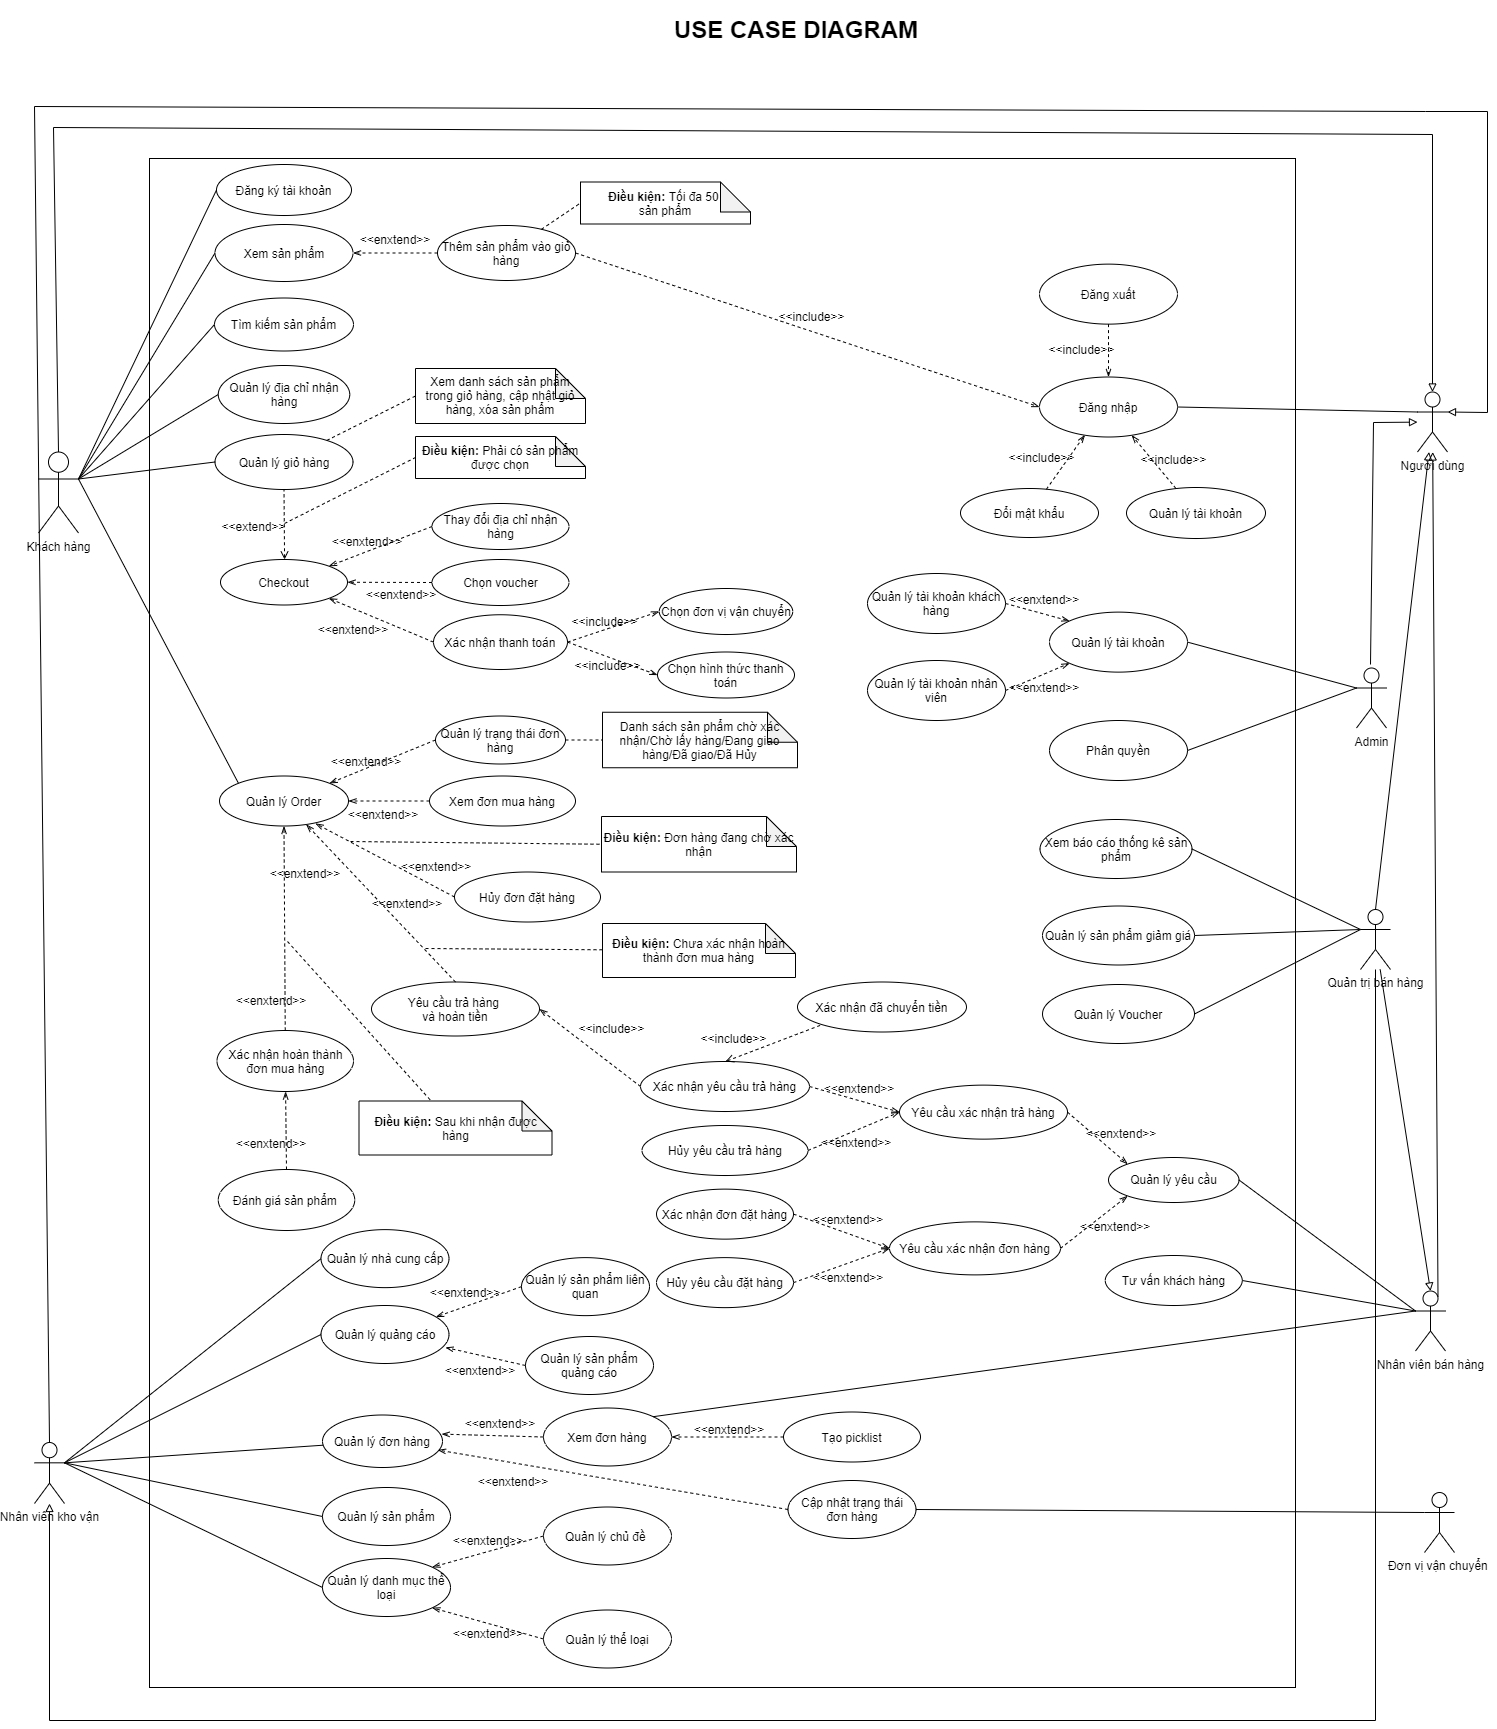
\includegraphics[width=1\linewidth]{lib/usecase/usecasediagram.png}\\\vspace*{1cm}
	\hspace{5cm}{Hình 1. Sơ đồ use case}\\
\subsection{Đặc tả use case}
\subsubsection{Đăng nhập}
    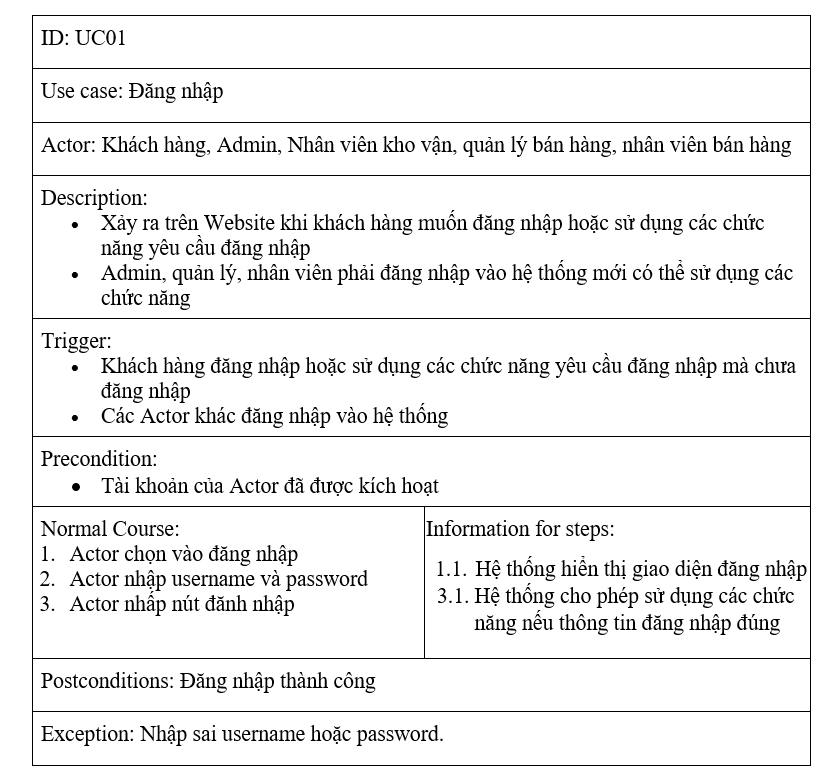
\includegraphics[width=1\linewidth]{lib/usecase/dangnhap.png}\\\vspace*{1cm}
\subsubsection{Đăng xuất}
    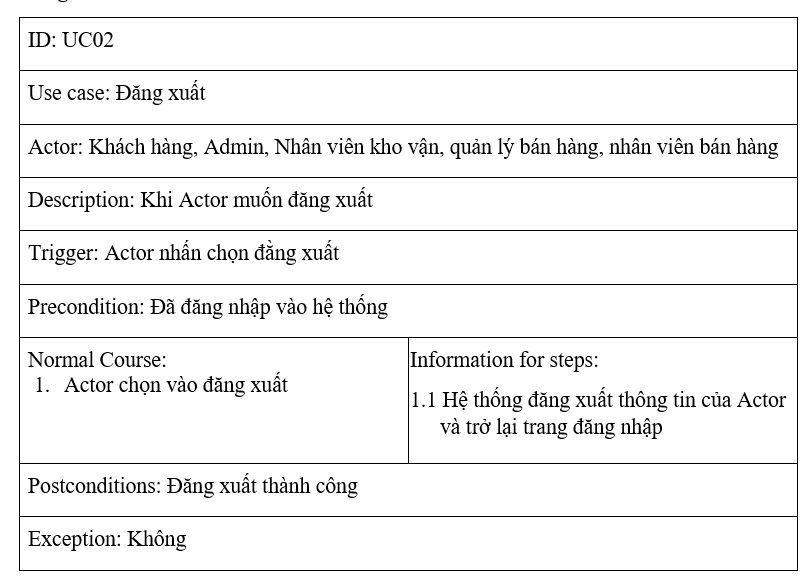
\includegraphics[width=1\linewidth]{lib/usecase/dangxuat.png}\\\vspace*{1cm}
\subsubsection{Xem sản phẩm vào giỏ hàng}
    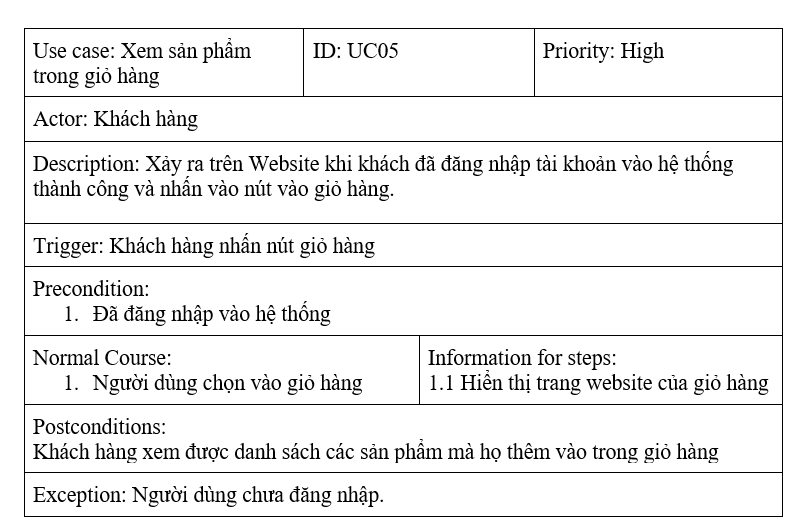
\includegraphics[width=1\linewidth]{lib/usecase/xemsp.png}\\\vspace*{1cm}
\subsubsection{Tìm kiếm sản phẩm}
    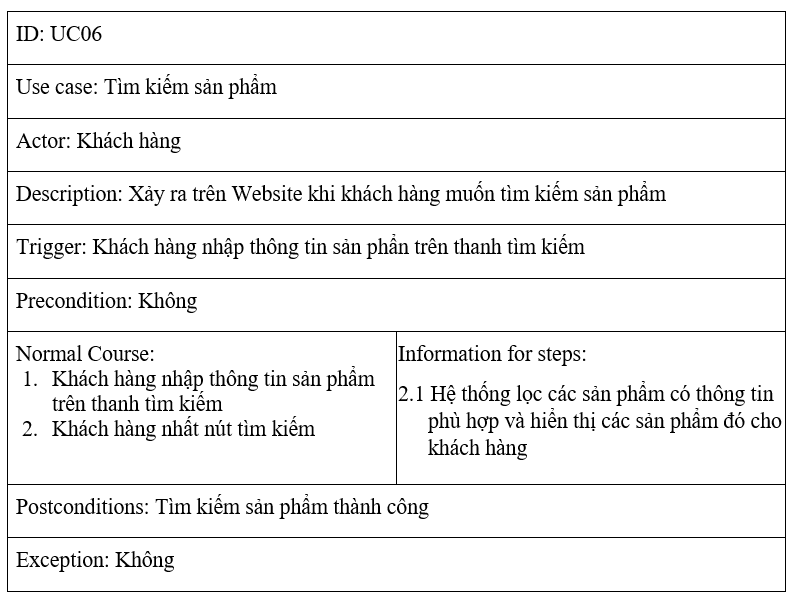
\includegraphics[width=1\linewidth]{lib/usecase/timkiemsp.png}\\\vspace*{1cm}
\subsubsection{Quản lý địa chỉ nhận hàng}
    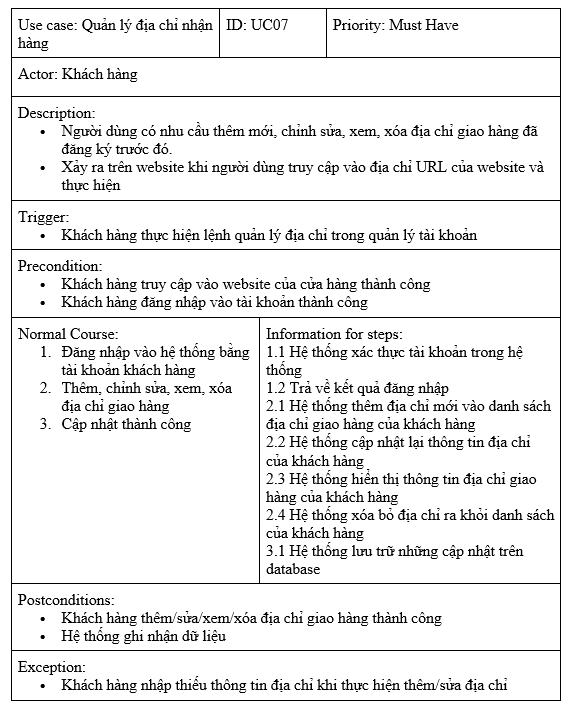
\includegraphics[width=1\linewidth]{lib/usecase/quanlydiachinh.png}\\\vspace*{1cm}
\subsubsection{Xem đơn hàng}
    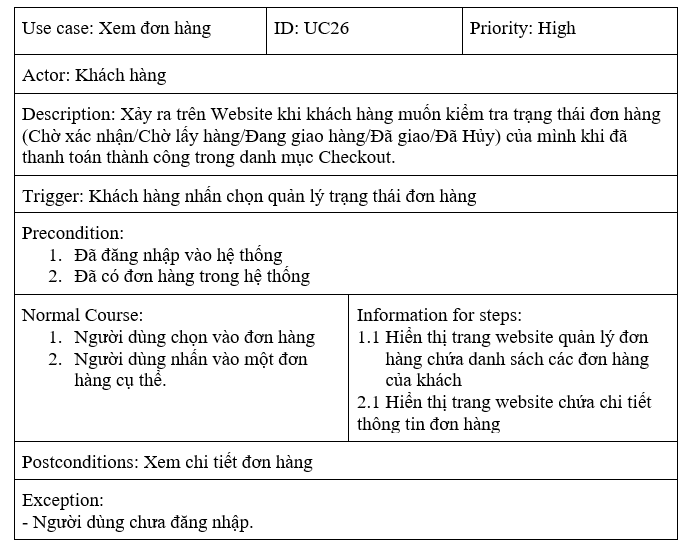
\includegraphics[width=1\linewidth]{lib/usecase/xemdonhang.png}\\\vspace*{1cm}
\subsubsection{Thêm sản phẩm vào giỏ hàng}
    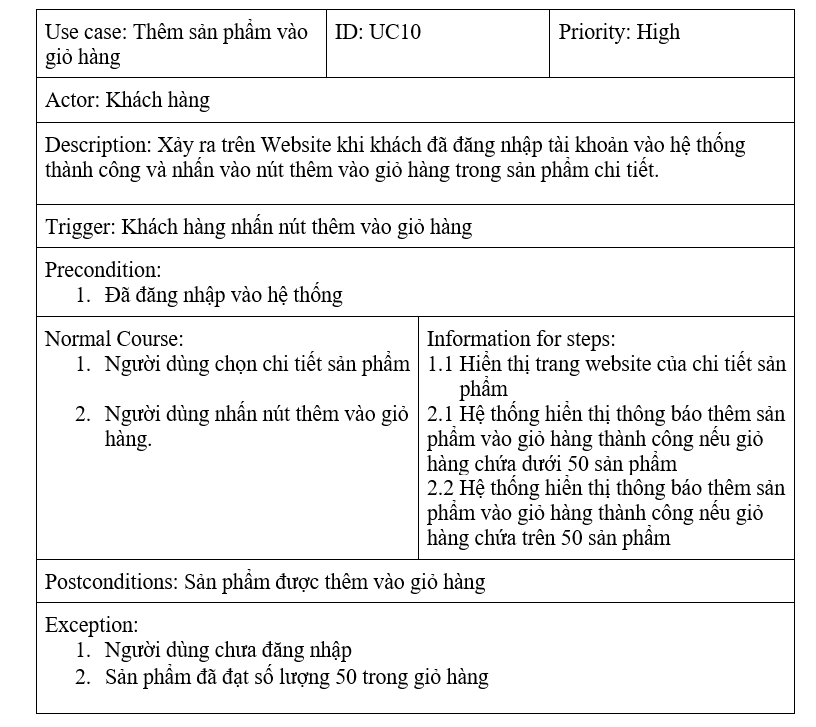
\includegraphics[width=1\linewidth]{lib/usecase/themspvaogio.png}\\\vspace*{1cm}
\subsubsection{Thay đổi địa chỉ nhận hàng}
    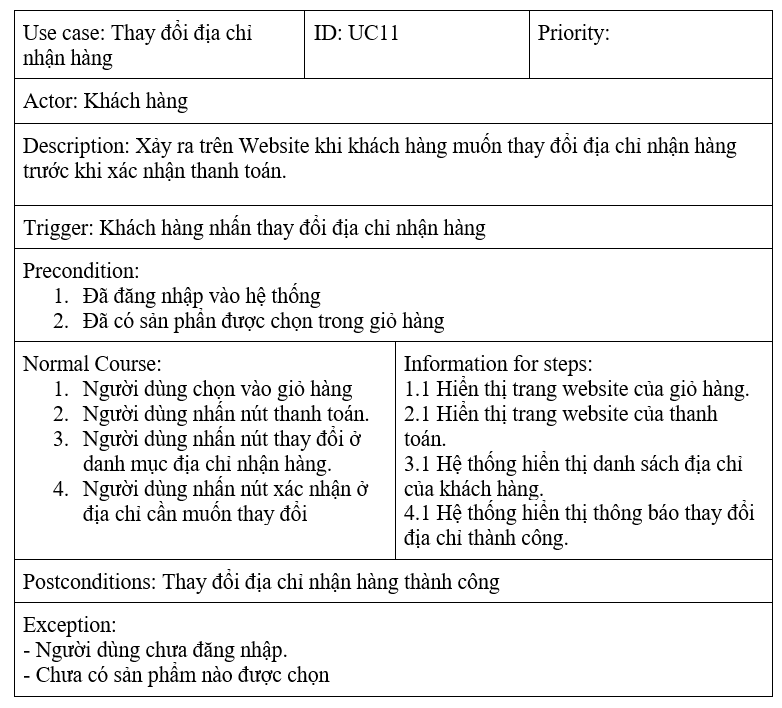
\includegraphics[width=1\linewidth]{lib/usecase/thaydoidiachiNh.png}\\\vspace*{1cm}
\subsubsection{Xác nhận thanh toán}
    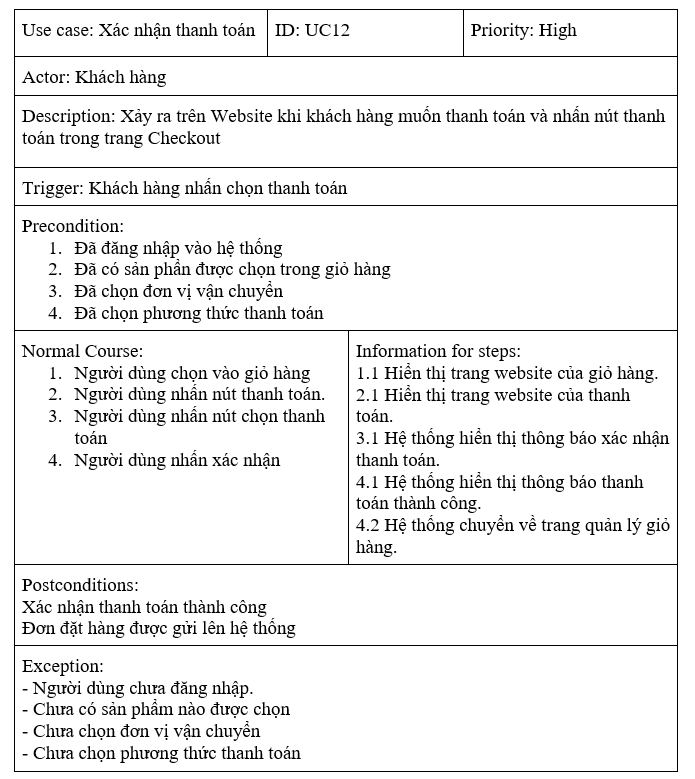
\includegraphics[width=1\linewidth]{lib/usecase/xacnhantt.png}\\\vspace*{1cm}
\subsubsection{Chọn đơn vị vận chuyển}
    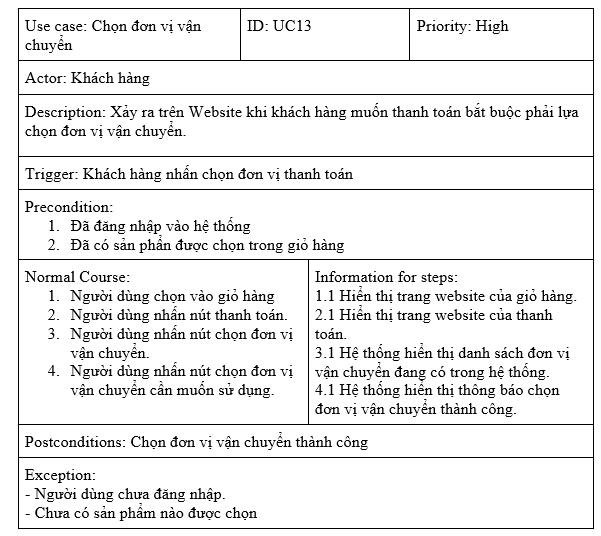
\includegraphics[width=1\linewidth]{lib/usecase/chondvvc.png}\\\vspace*{1cm}
\subsubsection{Chọn hình thức thanh toán}
    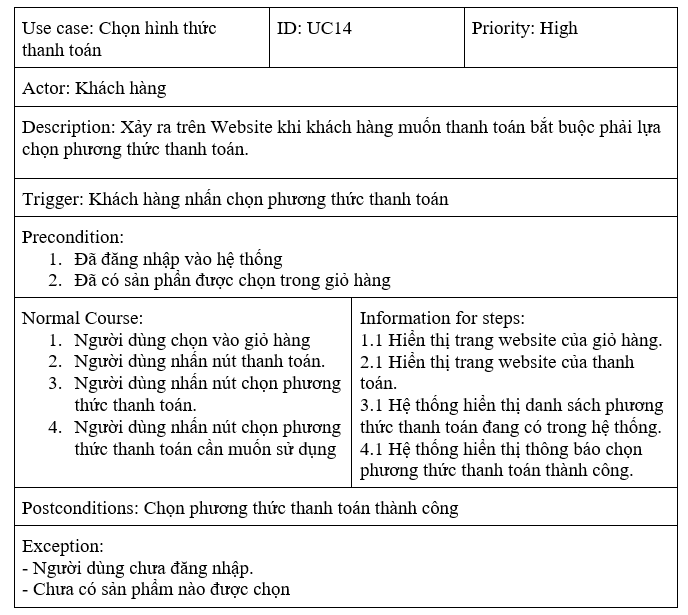
\includegraphics[width=1\linewidth]{lib/usecase/chonhttt.png}\\\vspace*{1cm}
\subsubsection{Chọn voucher}
    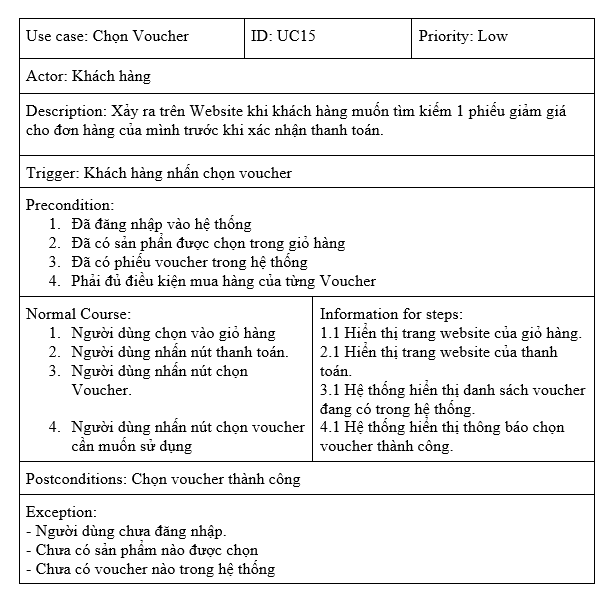
\includegraphics[width=1\linewidth]{lib/usecase/chonvoucher.png}\\\vspace*{1cm}
\subsubsection{Hủy đơn đặt hàng}
    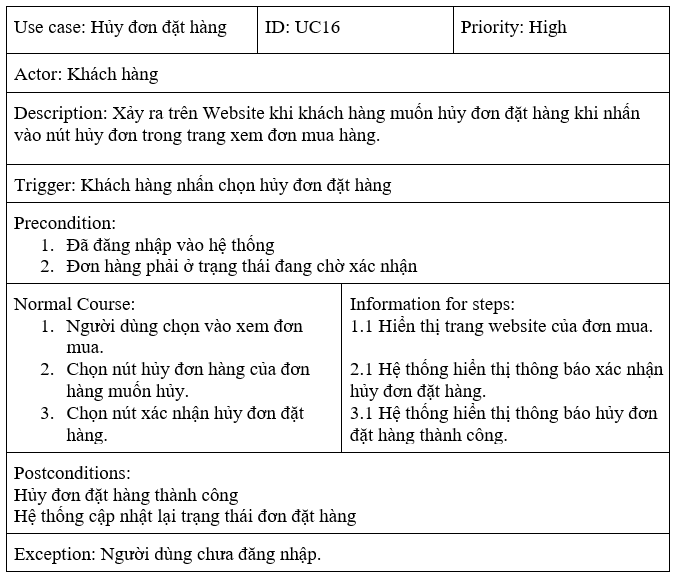
\includegraphics[width=1\linewidth]{lib/usecase/huydondat.png}\\\vspace*{1cm}
\subsubsection{Xem đơn mua hàng}
    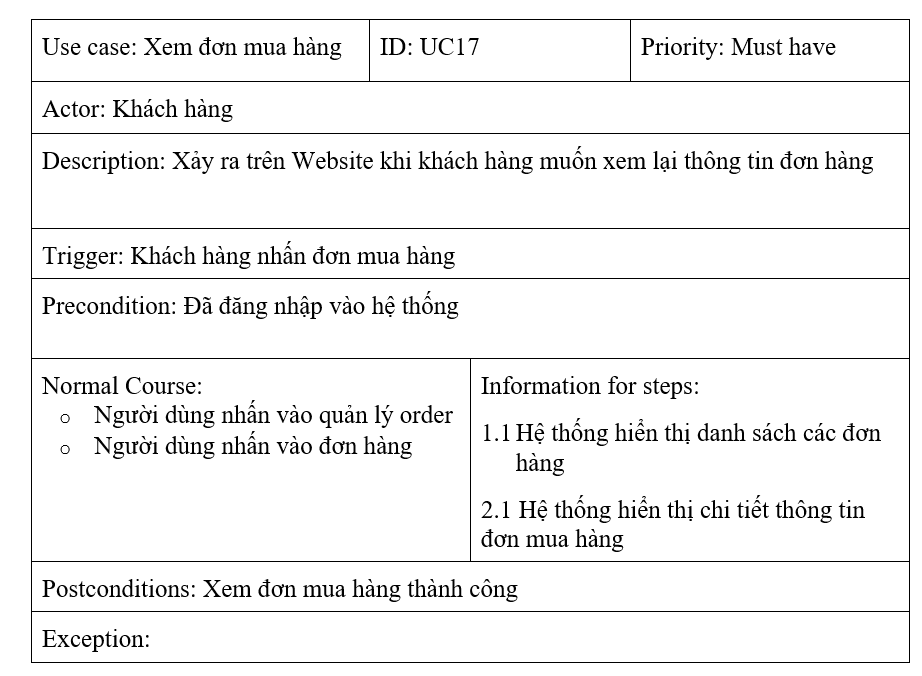
\includegraphics[width=1\linewidth]{lib/usecase/khachxemdon.png}\\\vspace*{1cm}    
\subsubsection{Yêu cầu trả hàng và hoàn tiền}
    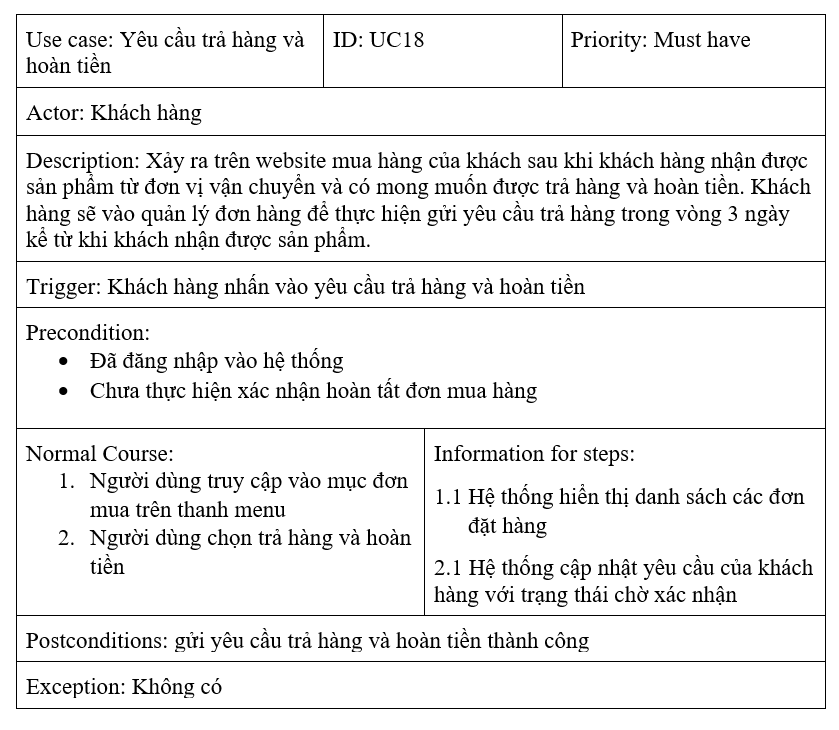
\includegraphics[width=1\linewidth]{lib/usecase/yeucautrahang.png}\\\vspace*{1cm}    
\subsubsection{Xác nhận hoàn tất đơn hàng}
    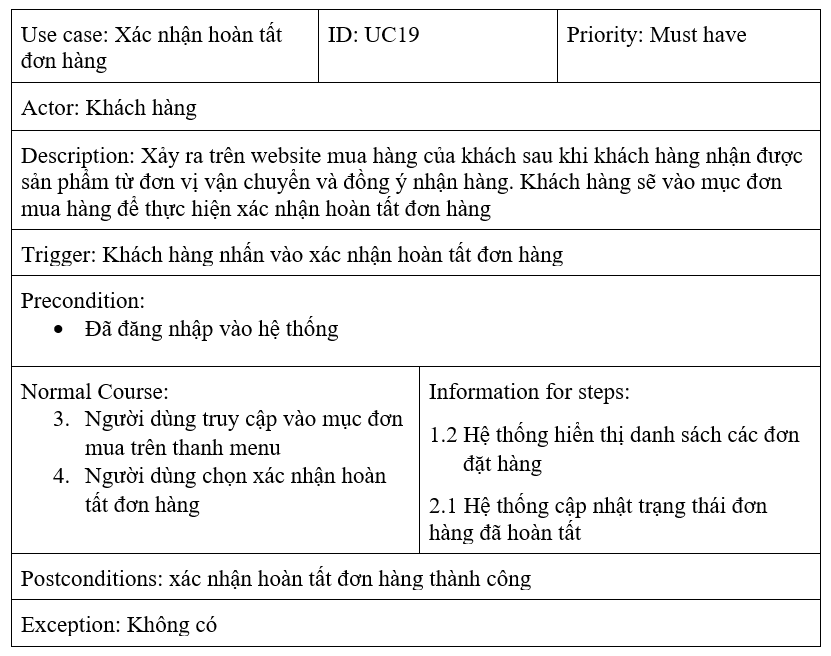
\includegraphics[width=1\linewidth]{lib/usecase/xacnhanhoantatdh.png}\\\vspace*{1cm}    
\subsubsection{Đánh giá sản phẩm}
    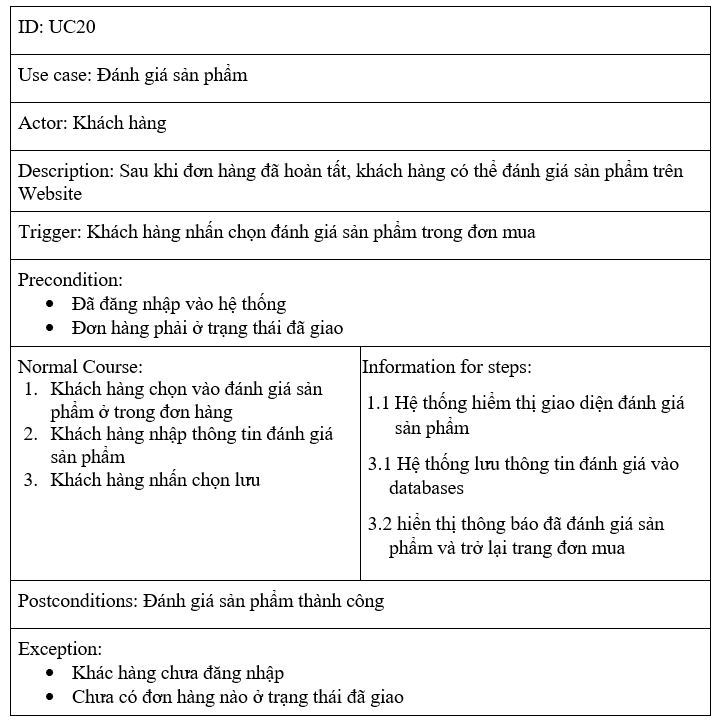
\includegraphics[width=1\linewidth]{lib/usecase/danhgiasp.png}\\\vspace*{1cm}    
\subsubsection{Quản lý giỏ hàng}
    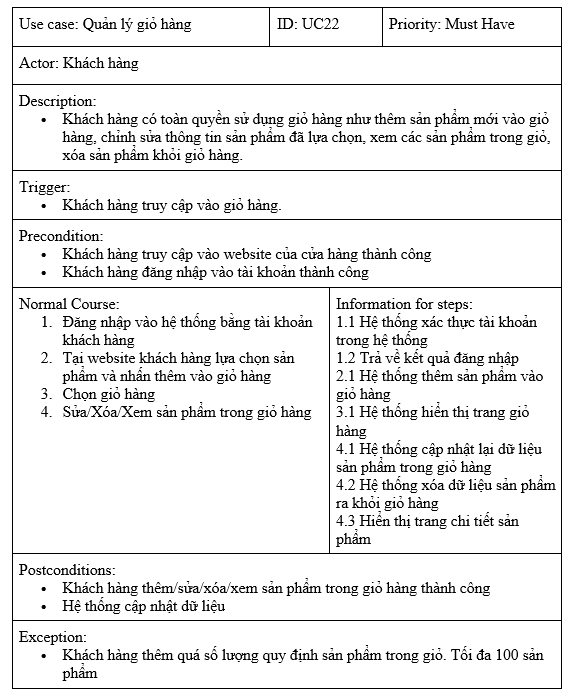
\includegraphics[width=1\linewidth]{lib/usecase/quanlygiohang.png}\\\vspace*{1cm}    
\subsubsection{Quản lý sản phẩm}
    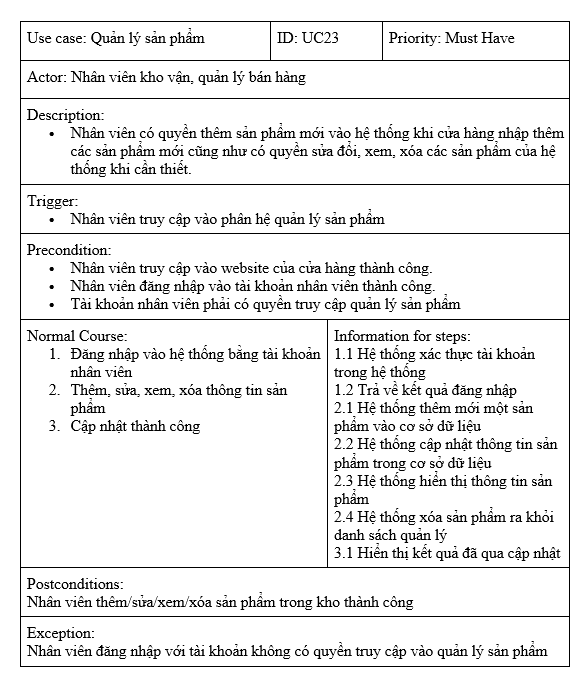
\includegraphics[width=1\linewidth]{lib/usecase/quanlysp.png}\\\vspace*{1cm}    
\subsubsection{Quản lý thể loại}
    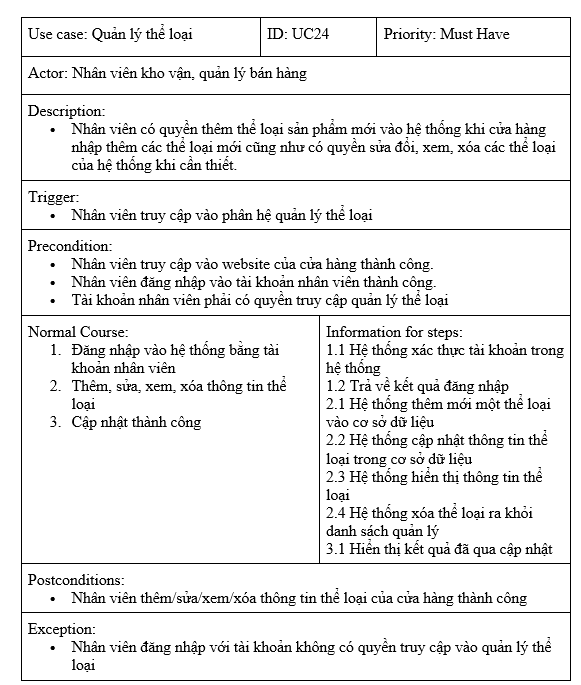
\includegraphics[width=1\linewidth]{lib/usecase/quanlytheloai.png}\\\vspace*{1cm}    
\subsubsection{Quản lý chủ đề}
    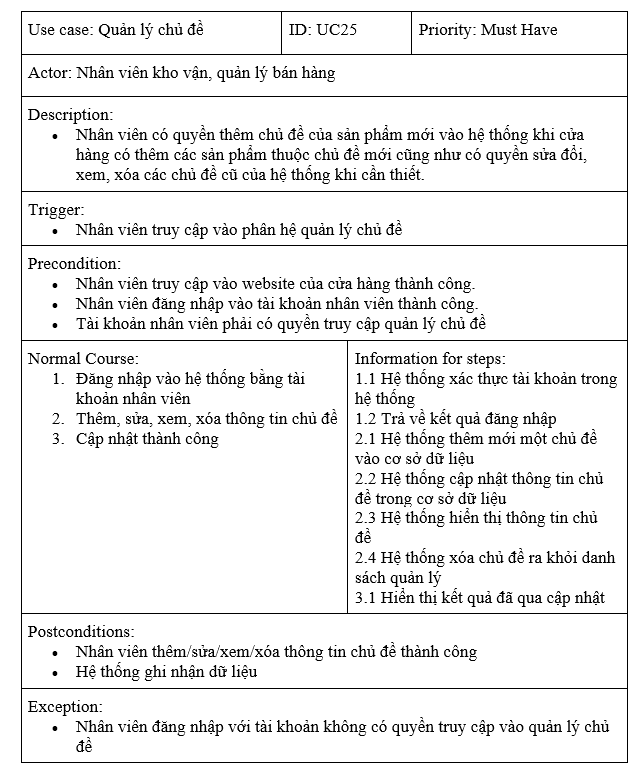
\includegraphics[width=1\linewidth]{lib/usecase/quanlychude.png}\\\vspace*{1cm}    
\subsubsection{Quản lý đơn hàng}
    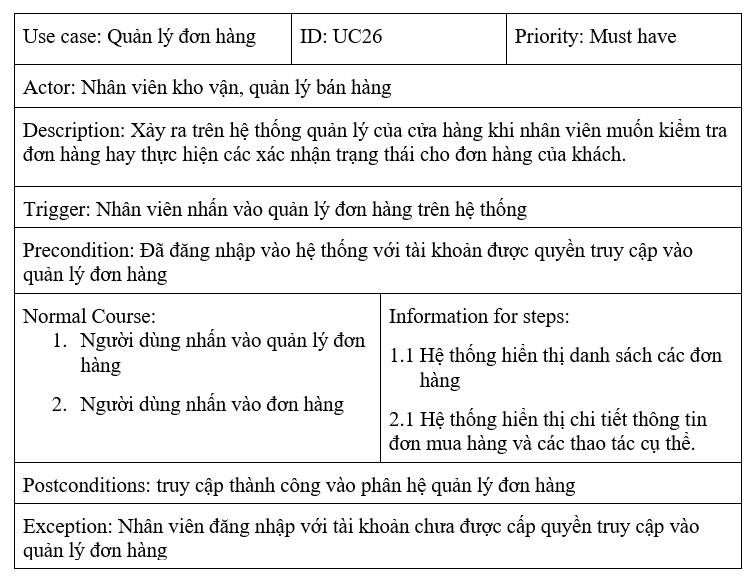
\includegraphics[width=1\linewidth]{lib/usecase/quanlydonhang.png}\\\vspace*{1cm}    
\subsubsection{Cập nhật trạng thái đơn hàng}
    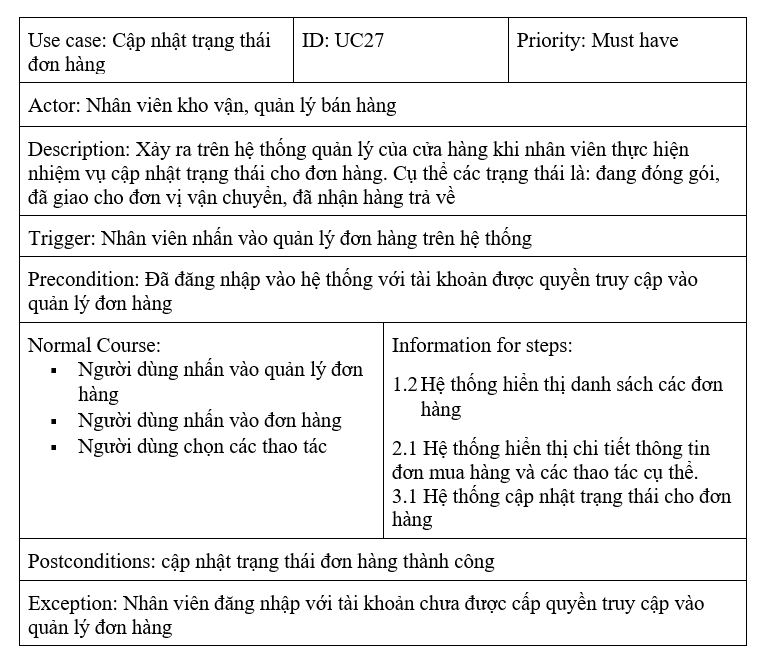
\includegraphics[width=1\linewidth]{lib/usecase/capnhattrangthaidh.png}\\\vspace*{1cm}    
\subsubsection{Quản lý nhà cung cấp}
    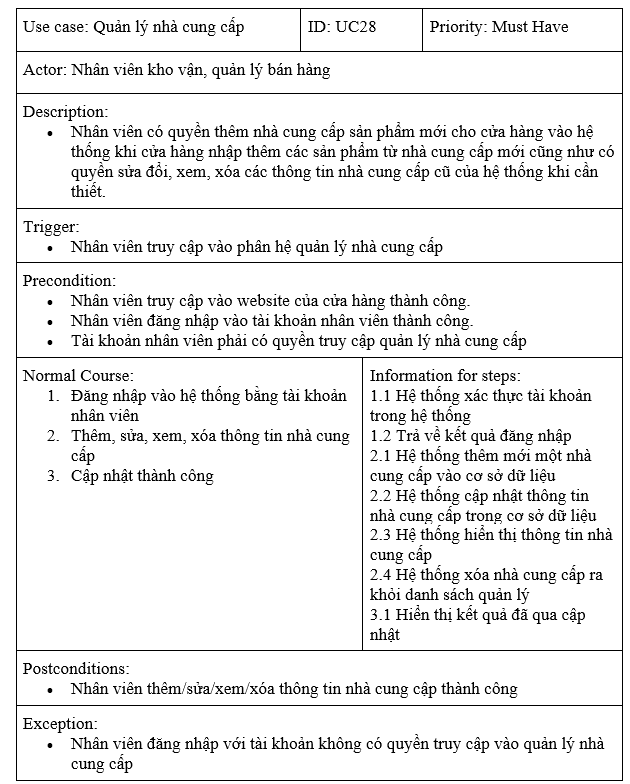
\includegraphics[width=1\linewidth]{lib/usecase/quanlyncc.png}\\\vspace*{1cm} 
\subsubsection{Quản lý sản phẩm liên quan}
    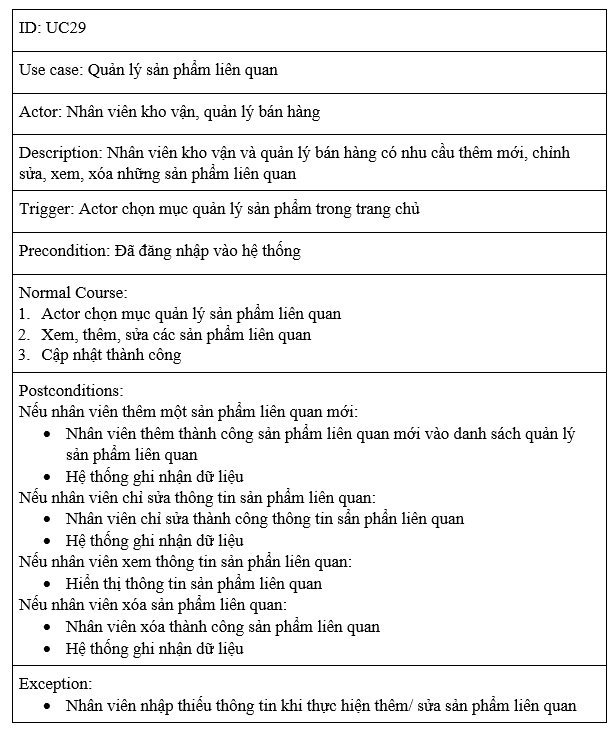
\includegraphics[width=1\linewidth]{lib/usecase/quanlysplienquan.png}\\\vspace*{1cm} 
\subsubsection{Xem đơn mua hàng}
    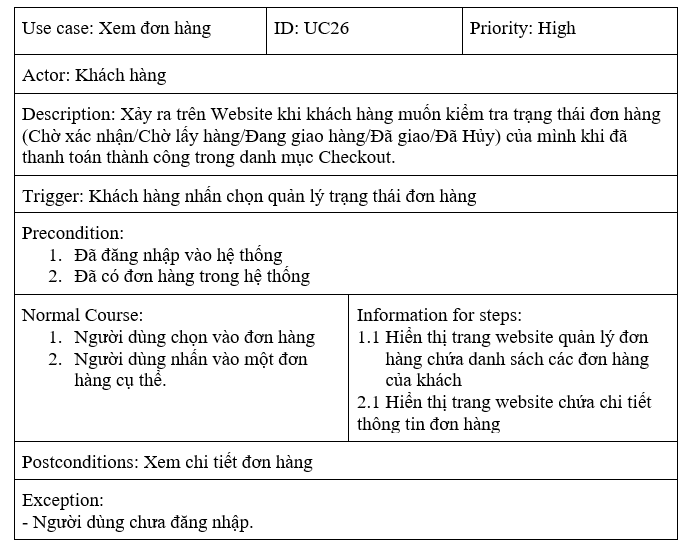
\includegraphics[width=1\linewidth]{lib/usecase/xemdonhang.png}\\\vspace*{1cm} 
\subsubsection{Yêu cầu xác nhận đơn đặt hàng}
    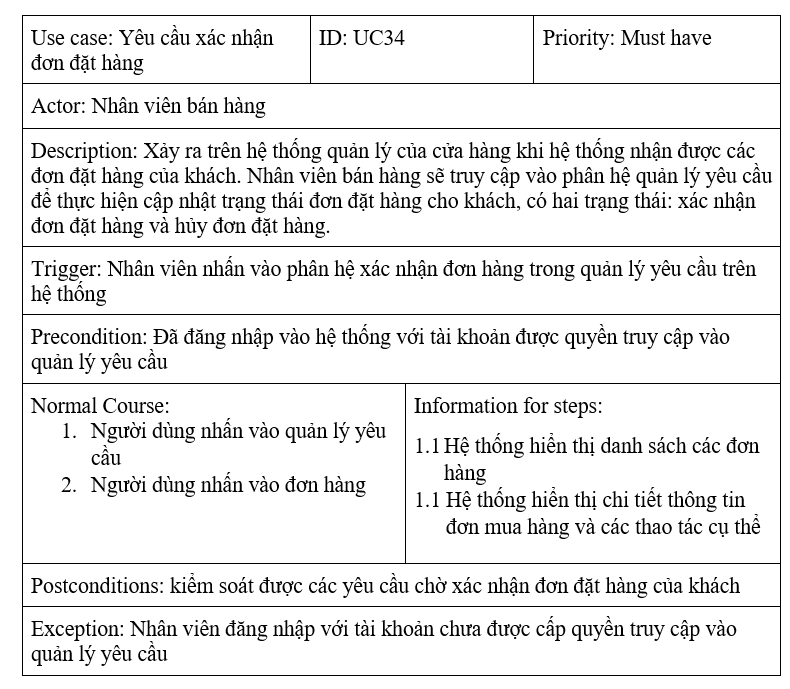
\includegraphics[width=1\linewidth]{lib/usecase/yeucauxacnhanddh.png}\\\vspace*{1cm} 
\subsubsection{Hủy yêu cầu đặt hàng}
    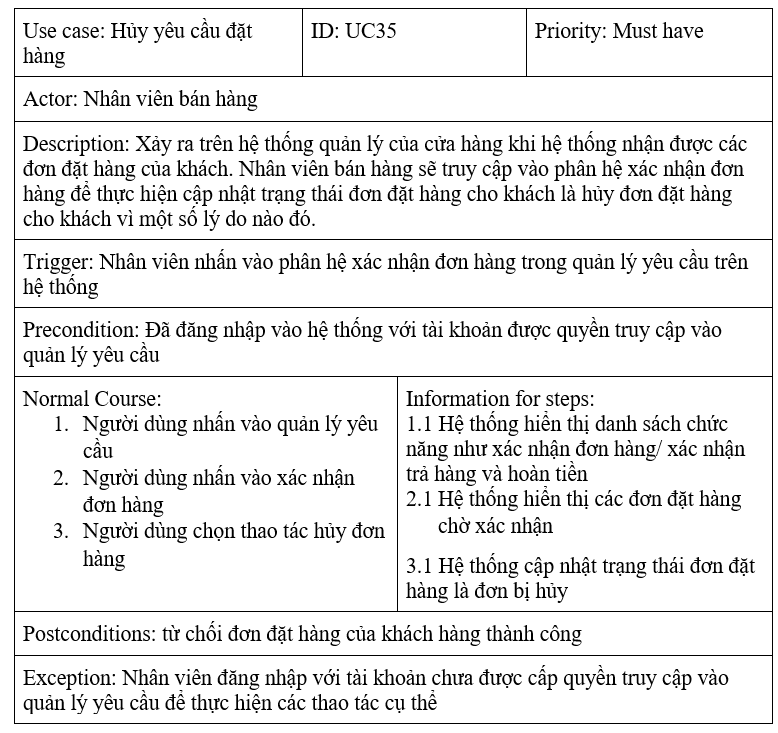
\includegraphics[width=1\linewidth]{lib/usecase/huyyeucaudh.png}\\\vspace*{1cm} 
\subsubsection{Xác nhận yêu cầu đặt hàng}
    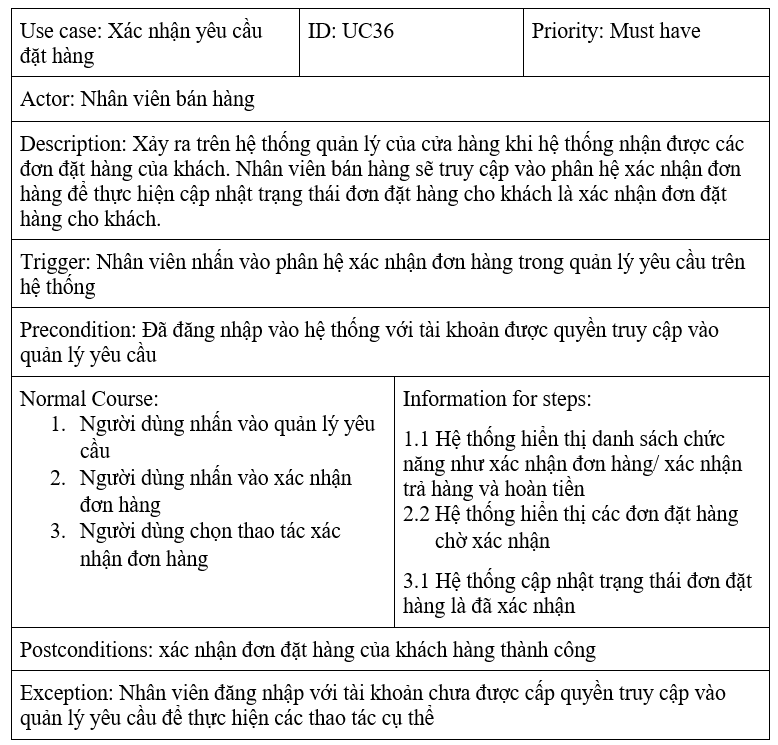
\includegraphics[width=1\linewidth]{lib/usecase/xacnhanyeucaudh.png}\\\vspace*{1cm} 
\subsubsection{Yêu cầu xác nhận trả hàng}
    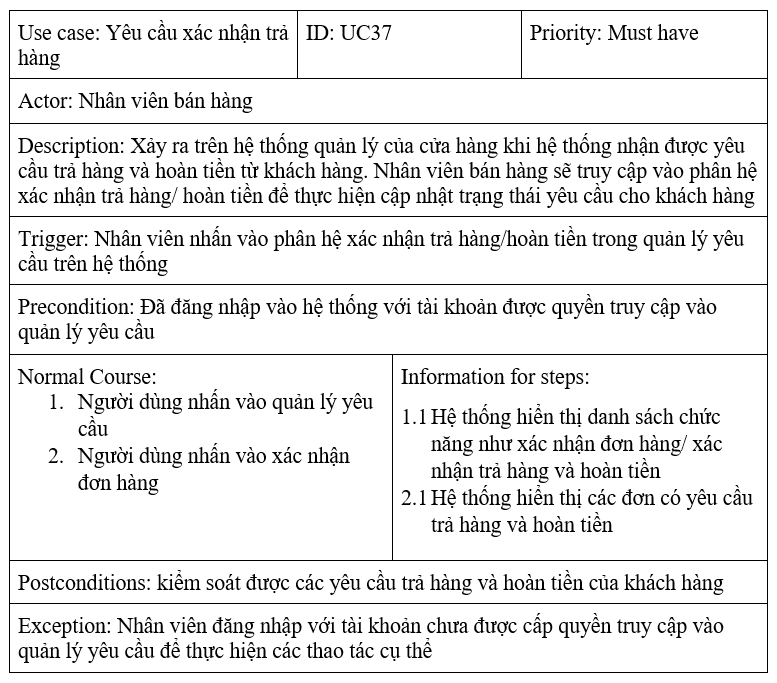
\includegraphics[width=1\linewidth]{lib/usecase/yeucauxacnhantrahang.png}\\\vspace*{1cm} 
\subsubsection{Xác nhận yêu cầu trả hàng và hoàn tiền}
    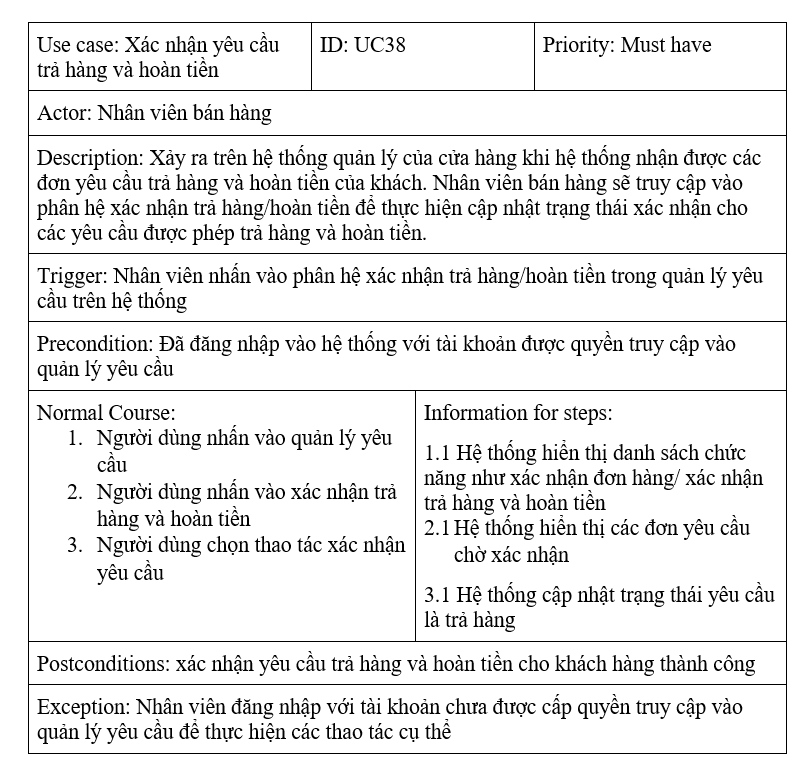
\includegraphics[width=1\linewidth]{lib/usecase/xacnhanyeucauth.png}\\\vspace*{1cm} 
\subsubsection{Hủy yêu cầu trả hàng và hoàn tiền}
    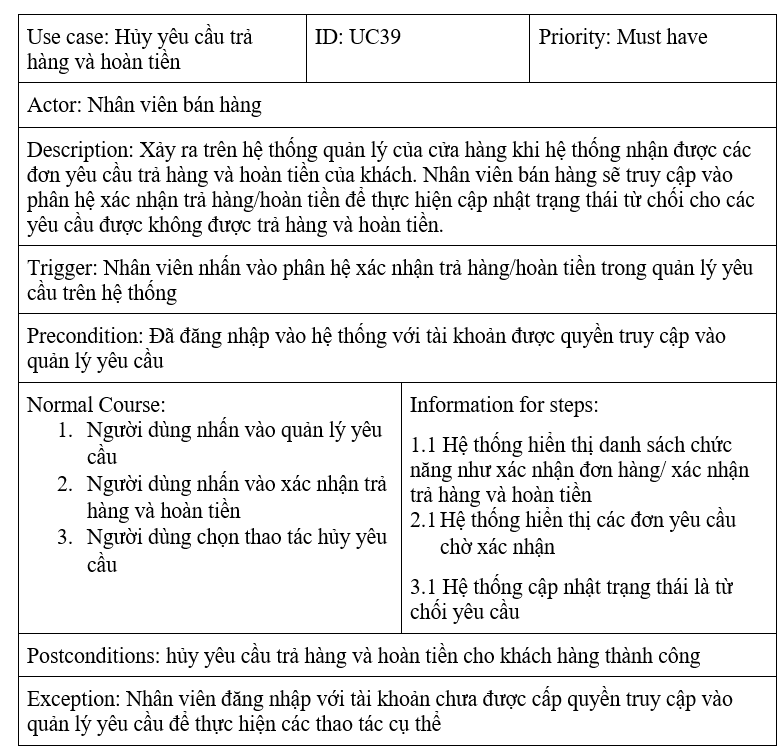
\includegraphics[width=1\linewidth]{lib/usecase/huyyeucauthvahoantien.png}\\\vspace*{1cm} 
\subsubsection{Quản lý voucher}
    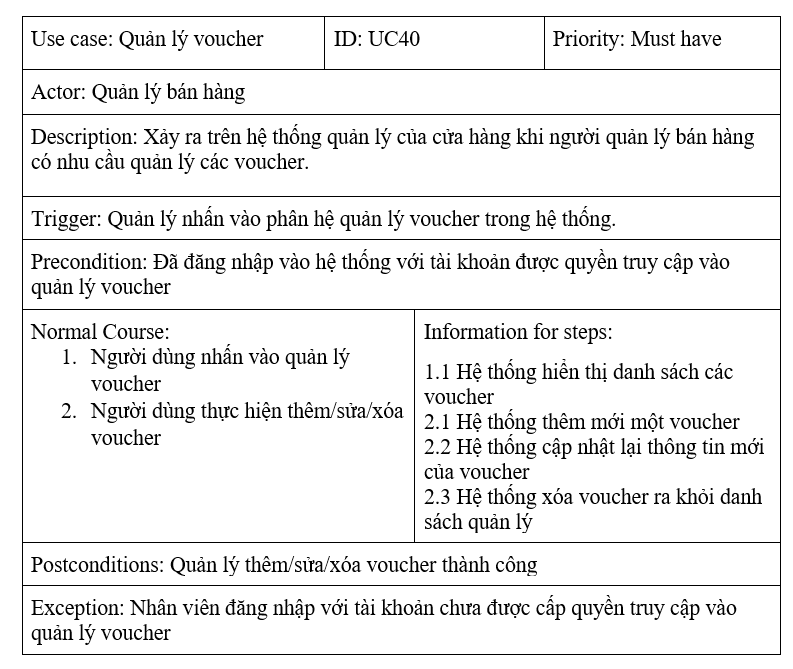
\includegraphics[width=1\linewidth]{lib/usecase/quanlyvoucher.png}\\\vspace*{1cm} 
\subsubsection{Quản lý giảm giá sản phẩm}
    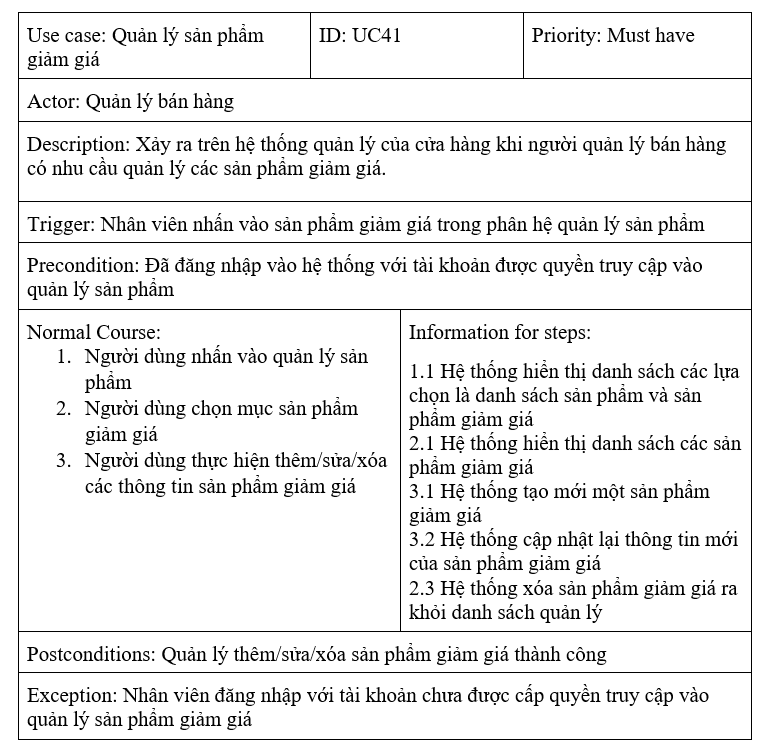
\includegraphics[width=1\linewidth]{lib/usecase/quanlyspgiamgia.png}\\\vspace*{1cm} 
\subsubsection{Quản lý tài khoản nhân viên}
    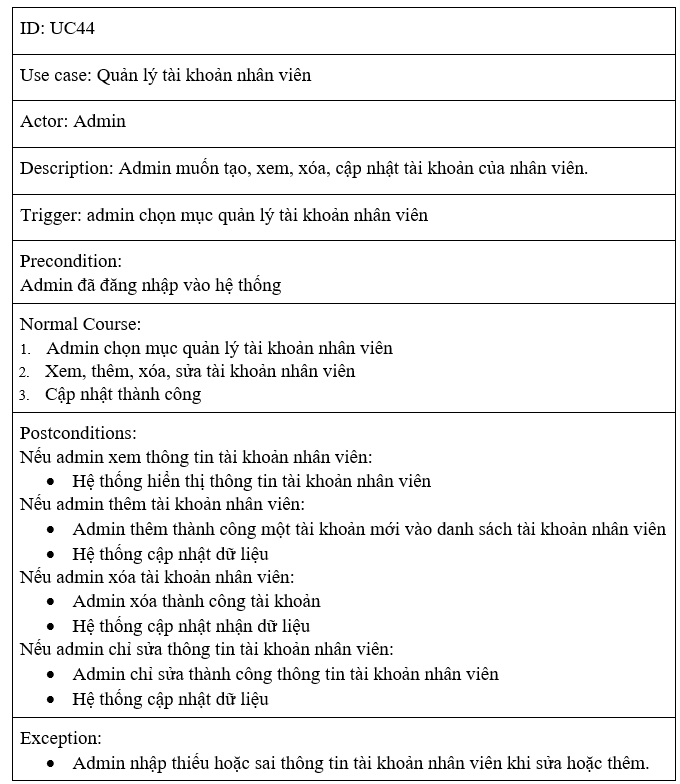
\includegraphics[width=1\linewidth]{lib/usecase/quanlytknv.png}\\\vspace*{1cm} 
\subsubsection{Quản lý tài khoản khách hàng}
    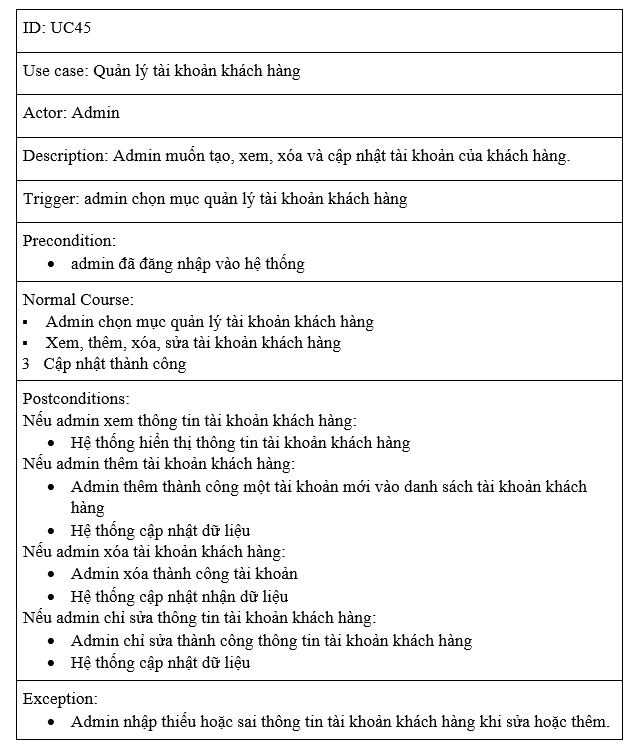
\includegraphics[width=1\linewidth]{lib/usecase/quanlytkkh.png}\\\vspace*{1cm} 
\subsection{Data Flow Diagram}
\subsubsection{2.3.3.1 Context Diagram}
    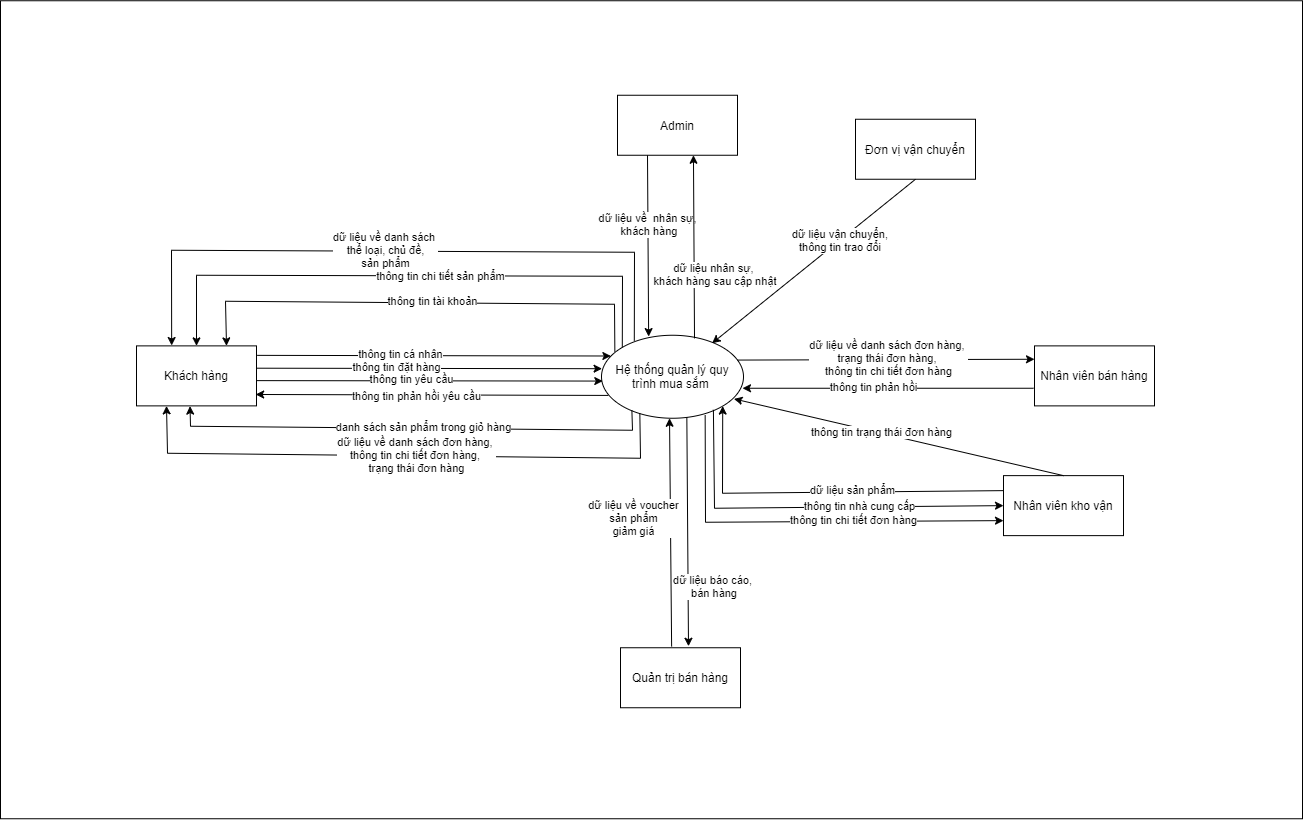
\includegraphics[width=1\linewidth]{lib/DFD/contextdi.png}\\\vspace*{1cm} 
    \hspace{5cm}{Hình 2. Context diagram}\\
\subsubsection{2.3.3.2 DFD Fragment}
    \subsubsection{Đăng nhập}
    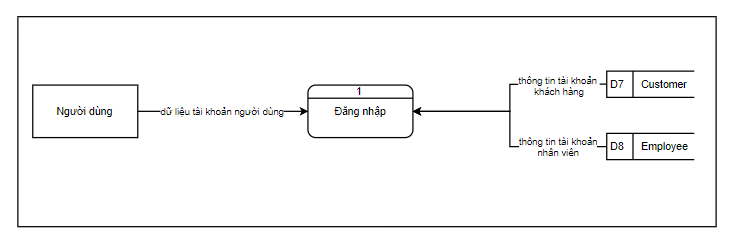
\includegraphics[width=1\linewidth]{lib/DFD/dangnhap.png}\\\vspace*{1cm}
    \hspace{5cm}{Hình 3. đăng nhập}\\
\subsubsection{Xem sản phẩm}
    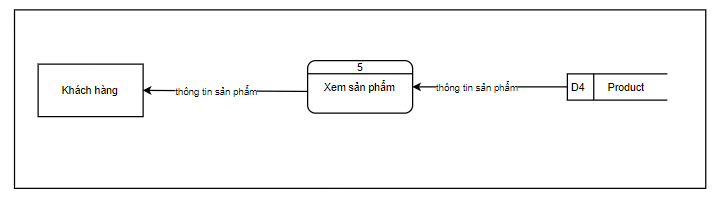
\includegraphics[width=1\linewidth]{lib/DFD/xemsp.png}\\\vspace*{1cm}
    \hspace{5cm}{Hình 4. Xem sản phẩm}\\
\subsubsection{Tìm kiếm sản phẩm}
    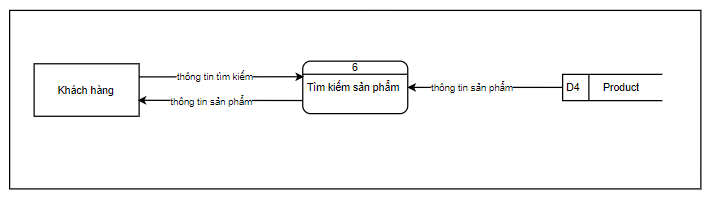
\includegraphics[width=1\linewidth]{lib/DFD/timkiemsp.png}\\\vspace*{1cm}
    \hspace{5cm}{Hình 5. Tìm kiếm sản phẩm}\\
\subsubsection{Quản lý địa chỉ nhận hàng}
    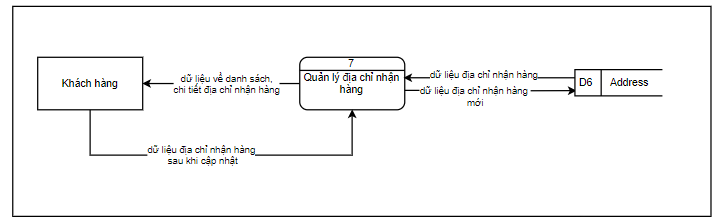
\includegraphics[width=1\linewidth]{lib/DFD/quanlydiachinh.png}\\\vspace*{1cm}
    \hspace{4cm}{Hình 6. Quản lý địa chỉ nhận hàng}\\
\subsubsection{Thêm sản phẩm vào giỏ hàng}
    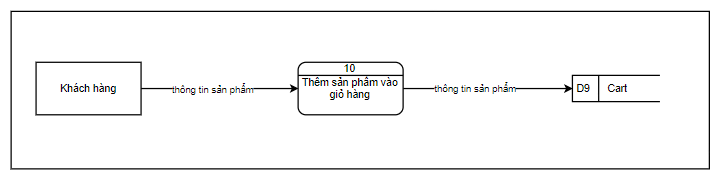
\includegraphics[width=1\linewidth]{lib/DFD/themspvaogio.png}\\\vspace*{1cm}
    \hspace{4cm}{Hình 7. Thêm sản phẩm vào giỏ hàng}\\
\subsubsection{Thay đổi địa chỉ nhận hàng}
    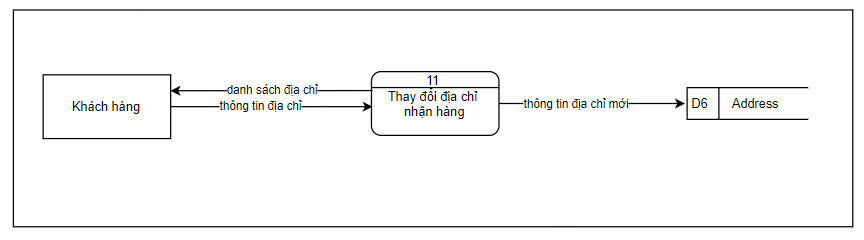
\includegraphics[width=1\linewidth]{lib/DFD/thaydoidiachinh.png}\\\vspace*{1cm}
    \hspace{4cm}{Hình 8. Thay đổi địa chỉ nhận hàng}\\
\subsubsection{Checkout}
    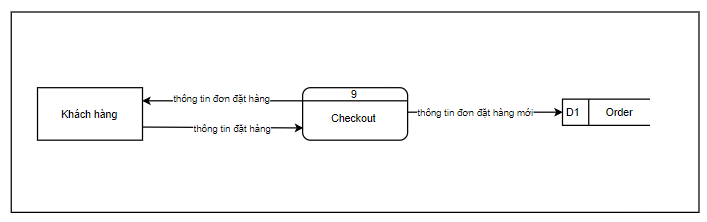
\includegraphics[width=1\linewidth]{lib/DFD/checkout.png}\\\vspace*{1cm}
    \hspace{5cm}{Hình 9. Checkout}\\
\subsubsection{Chọn đơn vị vận chuyển}
    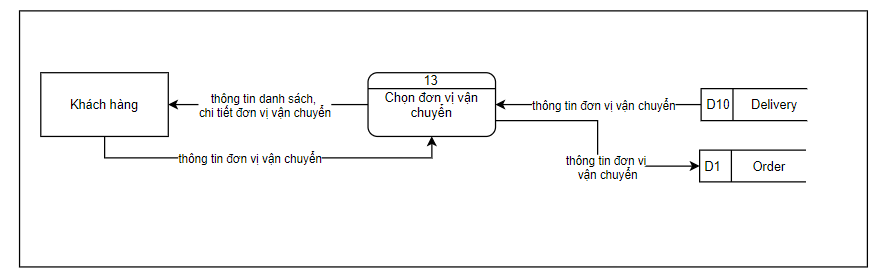
\includegraphics[width=1\linewidth]{lib/DFD/chondvvc.png}\\\vspace*{1cm}
    \hspace{4cm}{Hình 10. Chọn đơn vị vận chuyển}\\
\subsubsection{Chọn voucher}
    \includegraphics[width=1\linewidth]{lib/DFD/chonvoucher.png}\\\vspace*{1cm}
    \hspace{5cm}{Hình 11. Chọn voucher}\\
\subsubsection{Hủy đơn đặt hàng}
    \includegraphics[width=1\linewidth]{lib/DFD/huydondathang.png}\\\vspace*{1cm}
    \hspace{5cm}{Hình 12. Hủy đơn đặt hàng}\\
\subsubsection{Xem đơn mua hàng}
    \includegraphics[width=1\linewidth]{lib/DFD/xemdonmuahang.png}\\\vspace*{1cm} 
    \hspace{5cm}{Hình 13. Xem đơn mua hàng}\\
\subsubsection{Yêu cầu trả hàng và hoàn tiền}
    \includegraphics[width=1\linewidth]{lib/DFD/yeucautrahang.png}\\\vspace*{1cm}   
    \hspace{4cm}{Hình 14. Yêu cầu trả hàng và hoàn tiền}\\
\subsubsection{Xác nhận hoàn tất đơn hàng}
    \includegraphics[width=1\linewidth]{lib/DFD/xacnhanhoantatdh.png}\\\vspace*{1cm}  
    \hspace{4cm}{Hình 15. Xác nhận hoàn tất đơn hàng}\\
\subsubsection{Đánh giá sản phẩm}
    \includegraphics[width=1\linewidth]{lib/DFD/danhgiasp.png}\\\vspace*{1cm}  
    \hspace{5cm}{Hình 16. Đánh giá sản phẩm}\\
\subsubsection{Quản lý tài khoản}
    \includegraphics[width=1\linewidth]{lib/DFD/quanlytk.png}\\\vspace*{1cm}
    \hspace{5cm}{Hình 17. Quản lý tài khoản}\\
\subsubsection{Quản lý giỏ hàng}
    \includegraphics[width=1\linewidth]{lib/DFD/quanlygiohang.png}\\\vspace*{1cm}    
    \hspace{5cm}{Hình 18. Quản lý giỏ hàng}\\
\subsubsection{Quản lý sản phẩm}
    \includegraphics[width=1\linewidth]{lib/DFD/quanlysp.png}\\\vspace*{1cm}  
    \hspace{5cm}{Hình 19. Quản lý sản phẩm}\\
\subsubsection{Quản lý thể loại}
    \includegraphics[width=1\linewidth]{lib/DFD/quanlytheloai.png}\\\vspace*{1cm} 
    \hspace{5cm}{Hình 20. Quản lý thể loại}\\
\subsubsection{Quản lý chủ đề}
    \includegraphics[width=1\linewidth]{lib/DFD/quanlychude.png}\\\vspace*{1cm}    
    \hspace{5cm}{Hình 21. Quản lý chủ đề}\\
\subsubsection{Quản lý đơn hàng}
    \includegraphics[width=1\linewidth]{lib/DFD/quanlydonhang.png}\\\vspace*{1cm} 
    \hspace{5cm}{Hình 21. Quản lý đơn hàng}\\
\subsubsection{Cập nhật trạng thái đơn hàng}
    \includegraphics[width=1\linewidth]{lib/DFD/capnhattrangthaidh.png}\\\vspace*{1cm} 
    \hspace{4cm}{Hình 22. Cập nhật trạng thái đơn hàng}\\
\subsubsection{Quản lý nhà cung cấp}
    \includegraphics[width=1\linewidth]{lib/DFD/quanlynhacc.png}\\\vspace*{1cm} 
    \hspace{5cm}{Hình 23. Quản lý nhà cung cấp}\\
\subsubsection{Quản lý sản phẩm liên quan}
    \includegraphics[width=1\linewidth]{lib/DFD/quanlysplienquan.png}\\\vspace*{1cm} 
    \hspace{5cm}{Hình 24. Quản lý sản phẩm liên quan}\\
\subsubsection{Xác nhận yêu cầu đặt hàng}
    \includegraphics[width=1\linewidth]{lib/DFD/xacnhanyeucaudh.png}\\\vspace*{1cm} 
    \hspace{4cm}{Hình 25. Xác nhận yêu cầu đặt hàng}\\
\subsubsection{Yêu cầu xác nhận đơn đặt hàng}
    \includegraphics[width=1\linewidth]{lib/DFD/yeucauxacnhandonhang.png}\\\vspace*{1cm} 
    \hspace{4cm}{Hình 26. Yêu cầu xác nhận đơn đặt hàng}\\
\subsubsection{Hủy yêu cầu đặt hàng}
    \includegraphics[width=1\linewidth]{lib/DFD/huyyeucaudh.png}\\\vspace*{1cm} 
    \hspace{5cm}{Hình 27. Hủy yêu cầu đặt hàng}\\
\subsubsection{Yêu cầu xác nhận trả hàng}
    \includegraphics[width=1\linewidth]{lib/DFD/yeucauxacnhantrahg.png}\\\vspace*{1cm}
    \hspace{5cm}{Hình 28. Yêu cầu xác nhận trả hàng}\\
\subsubsection{Xác nhận yêu cầu trả hàng và hoàn tiền}
    \includegraphics[width=1\linewidth]{lib/DFD/xacnhanyeucautrahg.png}\\\vspace*{1cm} 
    \hspace{4cm}{Hình 29. Xác nhận yêu cầu trả hàng và hoàn tiền}\\
\subsubsection{Hủy yêu cầu trả hàng và hoàn tiền}
    \includegraphics[width=1\linewidth]{lib/DFD/huyyeucauth.png}\\\vspace*{1cm} 
    \hspace{4cm}{Hình 30. Xác nhận yêu cầu trả hàng và hoàn tiền}\\
\subsubsection{Quản lý voucher}
    \includegraphics[width=1\linewidth]{lib/DFD/quanlyvoucher.png}\\\vspace*{1cm} 
    \hspace{5cm}{Hình 31. Quản lý voucher}\\
\subsubsection{Quản lý giảm giá sản phẩm}
    \includegraphics[width=1\linewidth]{lib/DFD/quanlyspgiamgia.png}\\\vspace*{1cm} 
    \hspace{4cm}{Hình 32. Quản lý giảm giá sản phẩm}\\
 
\subsubsection{2.3.3.3 DFD level 0}
    \includegraphics[width=1\linewidth]{lib/DFD/level0.png}\\\vspace*{1cm} 
    \hspace{5cm}{Hình 33. DFD Level 0}\\
\chapter{Thiết kế cơ sở dữ liệu}
\section{Mô hình ERD}
    \includegraphics[width=1\linewidth]{lib/ERD.png}\\\vspace*{1cm} 
    \hspace{5cm}{Hình 34. Mô hình ERD}\\
\section{Lược đồ cơ sở dữ liệu}
    \includegraphics[width=1\linewidth]{lib/luocdocsdl.jpg}\\\vspace*{1cm} 
    \hspace{5cm}{Hình 35. Lược đồ cơ sở dữ liệu}\\
\chapter{Hiện thực phần mềm}
\section{Xác định quy trình phát triển phần mềm}
Hệ thống được thực hiện dựa trên mô hình thác nước (Waterfall model). Mô hình chia ra thành 6 giai đoạn chính như:
\begin{itemize}
    \item Phân tích yêu cầu: tìm hiểu và thu thập thông tin từ các nguồn có sẵn để nắm rõ quy trình nghiệp vụ
    \item Thiết kế hệ thống: theo yêu cầu để thiết kế các sơ đồ có liên quan
    \item Thực hiện: từ bản thiết kế tạo ra các chương trình phần mềm
    \item Thử nghiệm hệ thống: chắc chắn hệ thống đang hoạt động và chạy được trên môi trường tương ứng. 
    \item Bảo trì hệ thống: khắc phục các lỗi gặp phải trong quá trình thử nghiệm. Cập nhật các tính năng mới để hoàn thiện hệ thống
\end{itemize}
 \includegraphics[width=1\linewidth]{lib/Waterfall.png}\\\vspace*{1cm} 
\hspace{5cm}{Hình 36. Waterfall}\\
\section{Kế hoạch phát triển phần mềm}
\begin{itemize}
    \item Lập ý tưởng
    \item Tìm hiểu quy trình nghiệp vụ truyền thống
    \item Tìm hiểu quy trình nghiệp vụ hệ thống
    \item Phân tích yêu cầu: use case, đặc tả use case
    \item Thiết kế hệ thống: vẽ ERD - Entity Relationship Diagram và chuyển ERD sang lược đồ cơ sở dữ liệu, DFD level 0
    \item Hiện thực hệ thống: tiến hành xây dựng ứng dụng (bao gồm website giao diện người dùng và website dành cho cửa hàng)
    \item Tiến hành kiểm tra/đánh giá hệ thống
\end{itemize}
\section{Framework lập trình}

\hspace{0.7cm} Nhóm lựa chọn sử dụng framework Laravel được xây dựng trên nền PHP. Là framework có mã nguồn mở và miễn phí, được xây dựng để phát triển phần mềm, ứng dụng theo mô hình MVC. Hiện nay Laravel là PHP framework phổ biến nhất và tốt nhất, có độ tùy biến cao, hỗ trợ hiệu quả cho việc xây dựng các ứng dụng lớp và cần tốc độ xử lý nhanh như website thương mại điện tử, website bán hàng,...

Ưu điểm của Laravel:
\begin{itemize}
    \item Có nguồn tài liệu đầy đủ, rõ ràng
    \item Có nhiều thư viện, package được xây dựng bởi các lập trình viên trên khắp thế giới
    \item Bảo mật cao
    \item Tốc độ xử lý nhanh
    \item Tích hợp dễ dàng với các dịch vụ khác
    \item Khả năng tùy biến mạnh mẽ
\end{itemize}

Nhược điểm  của Laravel:
\begin{itemize}
    \item Thiếu sự liên kết giữa các phiên bản
    \item Cần có kỹ năng lập trình
\end{itemize}
\chapter{Kết quả sản phẩm}
\section{Trang thương mại điện tử}
\subsection{Trang bán hàng}
\subsubsection{Trang bán hàng}
    \includegraphics[width=1\linewidth]{lib/results/trangchu.jpg}\\\vspace*{1cm} 
    \hspace{5cm}{Hình 37. Trang chủ}\\
\subsubsection{Trang chi tiết sản phẩm}
    \includegraphics[width=1\linewidth]{lib/results/trangchitietsp.jpg}\\\vspace*{1cm}
    \hspace{5cm}{Hình 38. Trang chi tiết sản phẩm}\\
\subsubsection{Trang đăng nhập}
    \includegraphics[width=1\linewidth]{lib/results/login.jpg}\\\vspace*{1cm} 
    \hspace{5cm}{Hình 39. Trang đăng nhập}\\
\subsubsection{Trang đăng ký tài khoản}
    \includegraphics[width=1\linewidth]{lib/results/dangkytk.jpg}\\\vspace*{1cm}
    \hspace{5cm}{Hình 40. Trang đăng ký tài khoản}\\
\subsubsection{Trang giỏ hàng}
    \includegraphics[width=1\linewidth]{lib/results/giohang.jpg}\\\vspace*{1cm} 
    \hspace{5cm}{Hình 41. Trang giỏ hàng}\\
\subsubsection{Trang checkout}
    \includegraphics[width=1\linewidth]{lib/results/checkout.jpg}\\\vspace*{1cm} 
    \hspace{5cm}{Hình 42. Trang checkout}\\
\subsubsection{Trang quản lý đơn mua hàng}
    \includegraphics[width=1\linewidth]{lib/results/khquanlydonmua.jpg}\\\vspace*{1cm} 
    \hspace{5cm}{Hình 43. Trang quản lý đơn mua hàng}\\
\subsection{Trang quản lý của cửa hàng}
\subsubsection{Trang quản lý nhà cung cấp}
    \includegraphics[width=1\linewidth]{lib/results/quanlyncc.jpg}\\\vspace*{1cm}   
    \hspace{5cm}{Hình 44. Trang quản lý nhà cung cấp}\\
\subsubsection{Trang quản lý thuế}
    \includegraphics[width=1\linewidth]{lib/results/quanlythue.jpg}\\\vspace*{1cm}
    \hspace{5cm}{Hình 45. Trang quản lý thuế}\\
\subsubsection{Trang quản lý đơn vị vận chuyển}
    \includegraphics[width=1\linewidth]{lib/results/quanlydvvc.jpg}\\\vspace*{1cm} 
    \hspace{4cm}{Hình 46. Trang quản lý đơn vị vận chuyển}\\
\subsubsection{Trang quản lý voucher}
    \includegraphics[width=1\linewidth]{lib/results/quanlyvoucher.jpg}\\\vspace*{1cm}  
    \hspace{5cm}{Hình 47. Trang quản lý voucher}\\
\subsubsection{Trang quản lý thể loại}
    \includegraphics[width=1\linewidth]{lib/results/quanlytheloai.jpg}\\\vspace*{1cm}  
    \hspace{5cm}{Hình 48. Danh mục thể loại}\\
    \includegraphics[width=1\linewidth]{lib/results/quanlytheloai1.jpg}\\\vspace*{1cm} 
    \hspace{5cm}{Hình 49. Nhóm thể loại}\\
\subsubsection{Trang quản lý thuộc tính}
    \includegraphics[width=1\linewidth]{lib/results/kichthuocsp.jpg}\\\vspace*{1cm}  
    \hspace{5cm}{Hình 49. Quản lý kích thước sản phẩm}\\
    \includegraphics[width=1\linewidth]{lib/results/mausacsp.jpg}\\\vspace*{1cm}  
    \hspace{5cm}{Hình 50. Quản lý màu sắc sản phẩm}\\
\subsubsection{Trang quản lý sản phẩm}
    \includegraphics[width=1\linewidth]{lib/results/danhsachsp.jpg}\\\vspace*{1cm} 
    \hspace{5cm}{Hình 51. Danh sách sản phẩm}\\
    \includegraphics[width=1\linewidth]{lib/results/sanphamgiamgia.jpg}\\\vspace*{1cm}
    \hspace{5cm}{Hình 52. Quản lý sản phẩm giảm giá}\\
\subsubsection{Trang quản lý quảng cáo}
    \includegraphics[width=1\linewidth]{lib/results/splienquan.jpg}\\\vspace*{1cm}  
    \hspace{4cm}{Hình 53. Quản lý sản phẩm liên quan}\\
    \includegraphics[width=1\linewidth]{lib/results/spquangcao.jpg}\\\vspace*{1cm} 
    \hspace{4cm}{Hình 54. Quản lý sản phẩm cần quảng cáo}\\
\subsubsection{Trang quản lý yêu cầu}
    \includegraphics[width=1\linewidth]{lib/results/xacnhandonhang.jpg}\\\vspace*{1cm}  
    \hspace{4cm}{Hình 55. Danh sách các đơn hàng chờ duyệt}\\
    \includegraphics[width=1\linewidth]{lib/results/xacnhantrahang.jpg}\\\vspace*{1cm}  
    \hspace{3cm}{Hình 56. Danh sách các đơn hàng chờ duyệt trả hàng}\\
\subsubsection{Trang quản lý đơn hàng}
    \includegraphics[width=1\linewidth]{lib/results/cholayhang.jpg}\\\vspace*{1cm}  
    \hspace{5cm}{Hình 57. Các đơn chờ lấy }\\
    \includegraphics[width=1\linewidth]{lib/results/danggiao.jpg}\\\vspace*{1cm}  
    \hspace{5cm}{Hình 58. Các đơn hàng đang giao}\\
    \includegraphics[width=1\linewidth]{lib/results/dagiao.jpg}\\\vspace*{1cm}  
    \hspace{5cm}{Hình 59. Các đơn hàng đã giao}\\
    \includegraphics[width=1\linewidth]{lib/results/trahangvahoantien.jpg}\\\vspace*{1cm}  
    \hspace{4cm}{Hình 60. Các đơn trả hàng và hoàn tiền}\\
    \includegraphics[width=1\linewidth]{lib/results/donhangdahoantat.jpg}\\\vspace*{1cm}  
    \hspace{5cm}{Hình 61. Các đơn đã hoàn tất}\\
\subsubsection{Trang quản lý lịch sử thao tác}
    \includegraphics[width=1\linewidth]{lib/results/lichsuthaotac.jpg}\\\vspace*{1cm}  
    \hspace{5cm}{Hình 62. Quản lý lịch sử thao tác}\\
\section{Đánh giá}

Sau thời gian tìm hiểu về lý thuyết lẫn thực hành để hoàn thành đề tài “ Xây dựng và phát triển hệ thống quản lý quy trình mua sắm thời trang trực tuyến ”, nhóm chúng em đã tìm hiểu và học hỏi được những kiến thức mới cũng như ôn tập và vận dụng những kiến thức đã học. Cụ thể những kết quả mà nhóm đạt được như sau:

Hoàn thành được mục tiêu mong muốn ban đầu:
\begin{itemize}
    \item Tìm hiểu về quy trình mua sắm truyền thống
    \item Cải tiến quy trình truyền thống thành quy trình tự động
    \item Áp dụng kiến thức đã học để phân tích hệ thống
    \item Sử dụng kiến thức lập trình để thực thi hệ thống
\end{itemize}

Có thêm kiến thức về lập trình laravel, kiến thức và kỹ năng phân tích vấn đề cũng như phân tích hệ thống. Hệ thống được xây dựng trong đề tài này dưới dạng thực nghiệm là quản lý quy trình mua sắm của khách hàng. Mặc dù, đề tài này không còn mới mẻ tuy nhiên nó chính là tiền đề để chúng em có thể tiếp xúc và tìm hiểu thực tế về các vấn đề ngoài đời sống, những lợi ích mà thương mại điện tử mang lại cho con người. Chúng em được trải nghiệm và cùng nhau thực hiện phân tích và xây dựng trên những phần mềm phục vụ cho môn học

\section{Phân công, giao tiếp và đánh giá}
Thảo luận và quản lý đồ án:
\begin{itemize}
    \item Giao tiếp, thảo luận bằng messenger; họp mặt trên google meet
    \item Kế hoạch phân công được thông báo trên sheets hằng tuần
    \item Đồ án được thực hiện, chỉnh sửa và theo dõi cùng nhau trên một số nền tảng như: google docs, notion
    \item Khi hoàn thành xong, cả nhóm cùng nhau chỉnh sửa, đánh giá để hoàn thiện bài báo cáo.
\end{itemize}

\includegraphics[width=1\linewidth]{lib/phancong.png}\\\vspace*{1cm} 

\begin{thebibliography}{5}
	\bibitem{} Tài liệu học tập trường đại học Tôn Đức Thắng.
	\bibitem{} Alan Dennis, Barbara Haley Wixom, Roberta M. Roth, [2018], Systems Analysis and Design, 7th Edition, John Wiley & Sons, Inc., USA
\end{thebibliography}
\end{document}
